\documentclass[final]{foresj}

\nolinenumbers

\DOI{xxxxx}

\Year{2024}

\usepackage{listings}
\usepackage[dvipsnames]{xcolor}
% https://es.overleaf.com/learn/latex/Using_colors_in_LaTeX

\lstset{
  language=Matlab,
  basicstyle=\ttfamily\small,
  keywordstyle=\color{blue},
  commentstyle=\color{OliveGreen},
  stringstyle=\color{red},
  numberstyle=\tiny\color{gray},
  rulecolor=\color{black},
  breaklines=true,
  breakatwhitespace=true,
  showstringspaces=false,
}

\begin{document}

\title{Implementación de IoT en MATLAB para la Manipulación Robótica de un Robot SCARA}

\author[Implementación de IoT en MATLAB para la Manipulación
Robótica de un Robot SCARA]{Gabriel \surname{Hurtado Avilés}$^{2}$, Bryan \surname{Alatorre Marroquín}$^{1}$, José Manuel \surname{Villa Vargas}$^{1}$, Samyllerick \surname{Tapia Hernández}$^{1}$, Jorgue Miguel \surname{Jaimes Ponce}$^{1}$, José Antonio \surname{Lara Chavez}$^{1}$}

\address{$^{1}$Universidad Aut\'{o}noma Metropolitana, Unidad Azcapotzalco,~Ciudad de M\'{e}xico, M\'{e}xico\\
$^{2}$Universidad Nacional Autónoma de México, Facultad de Estudios Superiores Acatlán, Estado de México, México}

\corres{$^{\ast}$E-mail: gabrielhuav@gmail.com | Web: http://web.gabrielhuav.ovh/}

\date{\rec{23 de Mayo de 2024}}

\begin{abstract} Este reporte describe el desarrollo de un robot \textit{SCARA} (Selective Compliant Assembly Robot Arm) capaz de dibujar letras utilizando cinemática inversa en \textit{Matlab} con la librería \textit{Robotics Toolbox} de Peter Corke. El robot \textit{SCARA}, reconocido por su alta velocidad y precisión, se emplea comúnmente en aplicaciones de ensamblaje y manipulación de materiales. En este estudio, se explora su potencial para realizar tareas de dibujo precisas y repetitivas al implementar dos métodos para calcular las configuraciones articulares necesarias para que el efector final del robot alcance una posición y orientación deseadas: el método geométrico y el método \textit{Denavit-Hartenberg} (DH). El método DH, fundamental para la construcción del robot \textit{SCARA} en la biblioteca de robótica utilizada, se basa en la descripción sistemática de la estructura cinemática del robot mediante cuatro parámetros por eslabón: longitud, desplazamiento, ángulo de giro y ángulo de inclinación.
\break
\newline
Finalmente, se describe la implementación de un sistema de control para un robot \textit{SCARA} (Selective Compliant Assembly Robot Arm) con el objetivo de dibujar letras utilizando cinemática inversa y simulación. El proyecto integra diversos componentes como un microcontrolador \textit{ESP32}, una \textit{Raspberry Pi}, software \textit{Node-RED}, protocolo \textit{MQTT} y un dashboard gráfico. La simulación se realizó utilizando el entorno \textit{MATLAB Robotics Toolbox}, mientras que el control del robot real se implementó utilizando los componentes mencionados.
\break
\newline
\textbf{Palabras clave}: Robot SCARA, cinemática inversa, Robotics Toolbox, dibujo de letras, Matlab, IoT, MQTT, control de robots. 
\end{abstract}

\maketitle

\section{I. Introducción}

Los robots SCARA (Selective Compliant Assembly Robot Arm) son ampliamente utilizados en la industria por su precisión, velocidad y versatilidad en tareas como ensamblaje, Pick \& Place y manipulación de materiales. Su diseño compacto y ligero los hace ideales para aplicaciones que requieren movimientos rápidos y repetitivos en un espacio de trabajo limitado.

Estos autómatas son notablemente adaptables en su uso y se distinguen por su habilidad para operar a altas velocidades en tareas de Pick \& Place (trasladar y depositar componentes desde un lugar A hasta un destino B) y montaje. Usualmente poseen 4 grados de libertad (aunque algunos modelos cuentan con 3 ejes) y llevan a cabo labores con posicionamiento horizontal.

Operan con movimientos rotatorios en los ejes X e Y, y son inflexibles en el eje Z. Los robots SCARA son compactos y han sido concebidos para ejecutar labores exactas y reiterativas. Se emplean frecuentemente en aplicaciones de montaje, traslado y colocación, y manejo de materiales.

Hay una gran cantidad de productores que han creado su propio modelo de robot SCARA para satisfacer las necesidades de los diversos sectores industriales que se benefician de sus características. Por ejemplo, el productor de autómatas industriales KUKA presenta la serie KR 6 con dos modelos reducidos que proporcionan alta precisión para ciclos extremadamente rápidos. Otro productor, Fanuc, presenta los robots SR-3iA y SR-6iA, que cuentan con un diseño ultra reducido que les permite operar con alta exactitud.

\subsection{Características de los robots SCARA}

\begin{itemize}
\item Diseño compacto: Los robots SCARA son típicamente pequeños y livianos, lo que los hace ideales para aplicaciones que requieren espacios de trabajo reducidos.
\item Alta precisión: Los robots SCARA pueden alcanzar una alta precisión de posicionamiento, lo que los hace adecuados para tareas delicadas como el ensamblaje de componentes electrónicos.
\item Movimiento rápido: Los robots SCARA son capaces de realizar movimientos rápidos, lo que aumenta su productividad.
\item Bajo costo: Los robots SCARA son generalmente más económicos que otros tipos de robots industriales.
\end{itemize}

\section{II. Introducción a la Cinemática de Robots}

La cinemática en robótica se refiere al estudio del movimiento de los robots sin considerar las fuerzas y momentos involucrados. Se divide en dos ramas principales:

\begin{enumerate}
\item Cinemática directa: Calcula la posición y orientación del efector final a partir de los valores de las articulaciones (ángulos o distancias).
\item Cinemática inversa: Determina los valores angulares de las articulaciones necesarios para que el efector final alcance una posición y orientación deseadas.
\end{enumerate}

En el caso de los robots SCARA, la cinemática inversa es particularmente importante debido a la necesidad de controlar con precisión el movimiento del efector final para realizar tareas delicadas. Existen diversos métodos para resolver la cinemática inversa en robots SCARA. Algunos de los más comunes son:

\begin{itemize}
\item Método geométrico: Este método se basa en la aplicación de principios geométricos como el teorema de Pitágoras y la ley de los cosenos para determinar las articulaciones. Es un método relativamente sencillo pero puede ser computacionalmente costoso para robots con más grados de libertad.
\item Método de Denavit-Hartenberg (DH): Este método es un enfoque sistemático para describir la cinemática de robots articulados. Se define una serie de matrices de transformación homogénea que representan la relación entre los diferentes sistemas de coordenadas de los eslabones del robot. A partir de estas matrices, se pueden calcular las posiciones y orientaciones de cualquier punto del robot, incluyendo el efector final. El método DH es más complejo que el método geométrico, pero es más generalizable y eficiente para robots con múltiples grados de libertad.
\item Algoritmos iterativos: Existen diversos algoritmos iterativos que se pueden utilizar para resolver la cinemática inversa de robots SCARA. Estos algoritmos suelen ser más eficientes que los métodos geométricos y DH, especialmente para robots con un gran número de grados de libertad.
\end{itemize}

Es importante tener en cuenta que la cinemática inversa no siempre tiene una solución única. En algunos casos, puede haber múltiples conjuntos de ángulos articulares que resulten en la misma posición y orientación del efector final. Esto se conoce como el problema de la "degeneración cinemática". Además, la cinemática inversa no toma en cuenta las limitaciones físicas del robot, como los límites de rango de movimiento de las articulaciones. Por lo tanto, es importante verificar que las soluciones obtenidas sean cinemáticamente válidas y físicamente alcanzables.

\section{III. Diseño e Implementación de una Simulación y un Método en Matlab para Controlar el Robot}

La implementación de estos métodos en Matlab que se describe a continuación permite controlar con éxito el robot para dibujar letras. Los resultados demuestran la eficacia de la cinemática inversa en la programación de robots para realizar tareas complejas y precisas, contribuyendo así al avance en el campo de la robótica al demostrar la aplicación práctica de la cinemática inversa en el control de robots SCARA para realizar tareas de dibujo y escritura con precisión.

Antes de implementar un robot utilizando el método de Denavit-Hartenberg (DH), es importante realizar un análisis geométrico. El análisis geométrico implica entender la estructura física del robot y cómo sus componentes se conectan y se mueven entre sí. Esto incluye la identificación de los eslabones del robot, las articulaciones y los grados de libertad. También se debe entender cómo se mueven los eslabones y cómo las articulaciones permiten o restringen este movimiento. Por ejemplo, en nuestro robot SCARA, primero se identificaron los eslabones que se mueven en el plano horizontal (ejes X e Y) y el eslabón que se mueve en el plano vertical (eje Z). Posteriormente se analizó cómo las articulaciones rotacionales permiten el movimiento en los ejes X e Y, y cómo la articulación prismática permite el movimiento en el eje Z.

En la solución presentada, se utiliza la cinemática inversa para calcular los ángulos de las articulaciones necesarios para que el efector final del robot alcance una posición deseada en el espacio. Las ecuaciones clave que se utilizan en el análisis geométrico son:

\begin{itemize}
\item Ecuaciones de posición: Estas ecuaciones describen la posición de cada eslabón en el espacio. Para un eslabón i, la posición puede ser descrita por un vector de posición $$P_i$$
\item Ecuaciones de orientación: Estas ecuaciones describen la orientación de cada eslabón en el espacio. Para un eslabón i, la orientación puede ser descrita por una matriz de rotación $$R_i$$
\item Ecuaciones de transformación homogénea: Estas ecuaciones combinan las ecuaciones de posición y orientación en una sola matriz de 4x4 que describe tanto la posición como la orientación de cada eslabón en el espacio. Para un eslabón i, la matriz de transformación homogénea $$T_i$$ se puede escribir como: $$T_i = \begin{bmatrix} R_i & P_i \\ 0 & 1 \end{bmatrix}$$ Donde $$R_i$$ es la matriz de rotación y $$P_i$$ es el vector de posición
\item Ecuaciones de cinemática directa: Estas ecuaciones describen la posición y orientación del efector final (la “mano” del robot) en términos de las variables articulares. Estas ecuaciones se obtienen multiplicando las matrices de transformación homogénea de todos los eslabones.
\item Ecuaciones de cinemática inversa: Estas ecuaciones describen las variables articulares necesarias para que el efector final alcance una posición y orientación deseadas. Estas ecuaciones son más difíciles de obtener que las ecuaciones de cinemática directa.
\end{itemize}

\section{IV. Ecuaciones clave que se utilizan en el código de la solución implementada}

\subsection{Ecuaciones de los eslabones del robot SCARA}

Las ecuaciones de los eslabones del robot SCARA son las siguientes:

\begin{align*}
\text{Eslabón 1: } & L1 = \text{Link}([0, 0, 8, 0, 0]); \\
\text{Eslabón 2: } & L2 = \text{Link}([0, 0, 10, 0, 0]); \\
\text{Eslabón 3: } & L3 = \text{Link}([0, 0, 0, 0, 1]);
\end{align*}

\subsection{Ecuaciones para la trayectoria del robot}

Las ecuaciones para la trayectoria del robot son las siguientes:

\begin{align*}
\text{hx\_der}(i) &= -3; \\
\text{hy\_der}(i) &= -10 - \frac{14}{N} \cdot i; \\
\text{hz\_der}(i) &= 0;
\end{align*}

\subsection{Ecuaciones de cinemática inversa}

Las ecuaciones de cinemática inversa son las siguientes:

\begin{align*}
c2 &= \frac{x^2 + y^2 - L1^2 - L2^2}{2 \cdot L1 \cdot L2}; \\
\theta2 &= \arccos(c2); \\
k1 &= L1 + L2 \cdot \cos(\theta2); \\
k2 &= L2 \cdot \sin(\theta2); \\
\theta1 &= \arctan\left(\frac{y}{x}\right) - \arctan\left(\frac{k2}{k1}\right); \\
q1 &= \theta1; \\
q2 &= \theta2;
\end{align*}

Estas ecuaciones permiten calcular los ángulos de las articulaciones necesarios para que el efector final del robot alcance una posición deseada en el espacio.

\begin{figure}[ht]
\centering
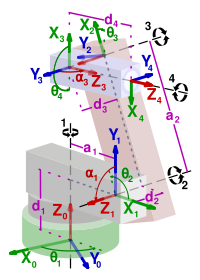
\includegraphics[width=0.3\textwidth]{DH.png}
\caption{Representación de las ecuaciones del método de Denavit-Hartenberg.}
\label{fig:my_label}
\end{figure}

Aunque estas ecuaciones permiten calcular los ángulos de las articulaciones necesarios para que el efector final del robot alcance una posición deseada en el espacio, es necesario resaltar que el método de Denavit-Hartenberg (DH) y el método geométrico son dos enfoques diferentes para resolver problemas de cinemática en robótica.

El método de Denavit-Hartenberg (DH) es una convención que se utiliza para definir de manera consistente los sistemas de coordenadas en un robot para facilitar la derivación de sus ecuaciones cinemáticas. Este método es particularmente útil para simplificar la descripción de la geometría de un robot, y es ampliamente utilizado en muchas librerías de robótica, incluyendo la librería Robotics Toolbox de Peter Corke, que es una herramienta muy útil para el estudio y la simulación de robots móviles y manipuladores de brazos de robots.

Esta librería proporciona muchas funciones útiles para la simulación de robótica clásica de tipo brazo, como la cinemática, la dinámica y la generación de trayectorias. Los objetos de robot pueden ser creados por el usuario para cualquier manipulador de enlace serial y se proporcionan varios ejemplos para robots conocidos de Kinova, Universal Robotics, Rethink, así como robots clásicos como el Puma 560 y el brazo de Stanford.

La librería contiene funciones y clases para representar la orientación y la posición en 2D y 3D (SO(2), SE(2), SO(3), SE(3)) como matrices, cuaterniones, giros, ángulos triples y exponenciales de matrices1. También proporciona funciones para manipular y convertir entre tipos de datos como vectores, transformaciones homogéneas y cuaterniones unitarios, que son necesarios para representar la posición y orientación tridimensional.

Específicamente, la librería Robotics Toolbox de Peter Corke utiliza el método de Denavit-Hartenberg (DH) para representar la cinemática de manipuladores de enlace serial como objetos de MATLAB. En la librería, cada eslabón del robot se define mediante una serie de parámetros DH, que luego se utilizan para calcular la matriz de transformación homogénea para ese eslabón. Esta matriz de transformación se utiliza para calcular la posición y orientación del eslabón en el espacio1. Por ejemplo, en el código de la solución, los eslabones del robot SCARA se definen utilizando la función Link de la librería, que toma como argumentos los parámetros DH del eslabón. Luego, se utiliza la función SerialLink para crear un objeto de robot que consta de estos eslabones.

El método DH es fundamental para la librería Robotics Toolbox porque proporciona una forma sistemática y consistente de definir los sistemas de coordenadas en un robot, lo que facilita la derivación de sus ecuaciones cinemáticas. En el método DH, cada eslabón del robot se define mediante una serie de parámetros DH, que luego se utilizan para calcular la matriz de transformación homogénea para ese eslabón. La matriz de transformación homogénea DH se define como: 
\[
T_{i-1}^i =
\]
\[
\begin{bmatrix} \cos(\theta_i) & -\sin(\theta_i)\cos(\alpha_{i-1}) & \sin(\theta_i)\sin(\alpha_{i-1}) & r_{i-1}\cos(\theta_i) \\ \sin(\theta_i) & \cos(\theta_i)\cos(\alpha_{i-1}) & -\cos(\theta_i)\sin(\alpha_{i-1}) & r_{i-1}\sin(\theta_i) \\ 0 & \sin(\alpha_{i-1}) & \cos(\alpha_{i-1}) & d_{i-1} \\ 0 & 0 & 0 & 1 \end{bmatrix}
\]

Por otro lado, el método geométrico se utiliza para resolver el problema de cinemática inversa que implican encontrar las variables articulares que resultan en una posición y orientación deseadas del efector final del robot.

\section{V. Simulación y Codificación de un Robot tipo SCARA en Matlab y Matlab Online}

En la solución inicial propuesta se utiliza el método geométrico para calcular los ángulos de las articulaciones necesarios para que el efector final del robot SCARA alcance una posición deseada en el espacio.

El uso de la cinemática inversa, que implica calcular las configuraciones articulares necesarias para que el efector final del robot alcance una posición y orientación deseadas, ha sido fundamental para lograr este objetivo. A través de la implementación de este concepto en Matlab, se ha logrado controlar con éxito el robot para dibujar las letras G, H y A. El procedimiento para realizar la tarea se puede resumir en los siguientes pasos:

\begin{enumerate}
\item Definición del robot y espacio de trabajo.
\item Dibujo de la letra G, H y A.
\item Controles para actualizar la posición del robot.
\item Función de cinemática inversa.
\end{enumerate}

En las siguiente figuras, se visualiza la simulación al ejecutar el código, como se observa, se calculan las trayectorias para cada segmento de las letras con líneas rectas y semicírculos. Se utilizan las funciones \texttt{inverse\_kinematics} y \texttt{plot\_sphere} para dibujar las trayectorias y el robot.

\begin{figure}[h!]
\centering
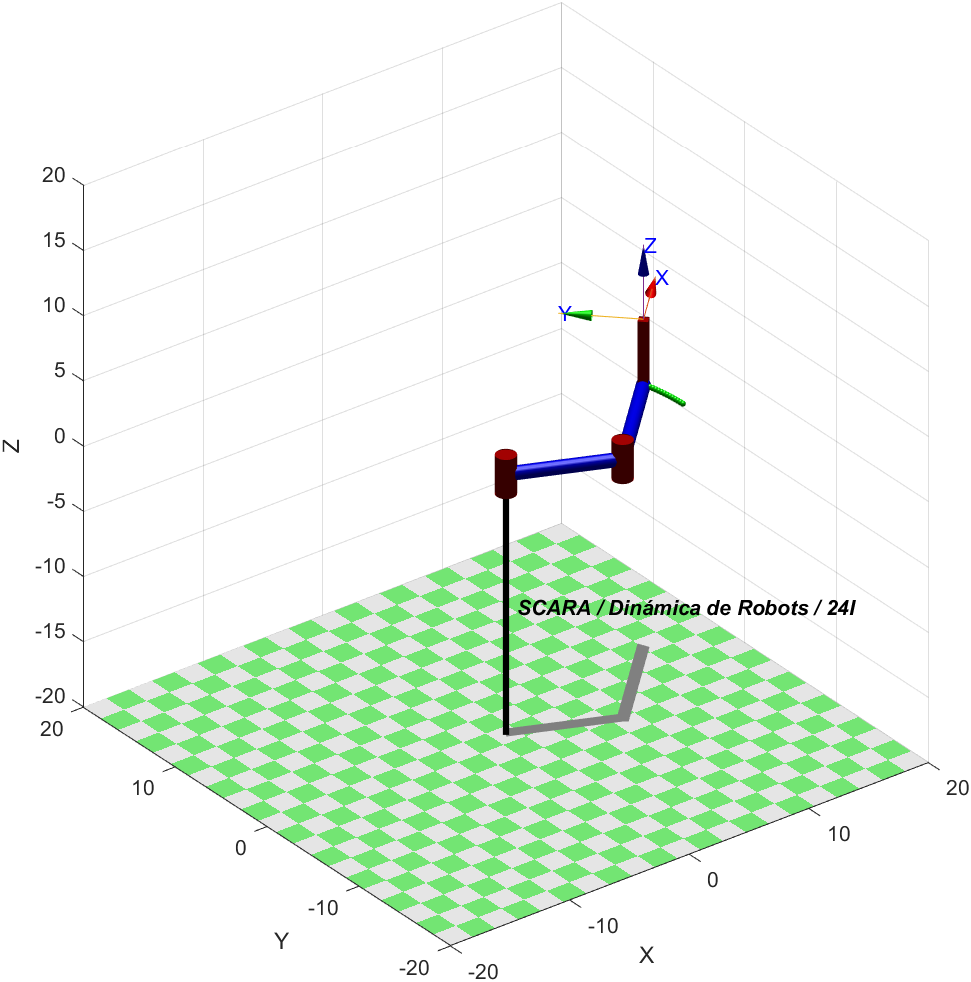
\includegraphics[width=0.5\textwidth]{G0.png}
\caption{Ilustración No. 1 de la Simulación.}
\label{fig:my_label}
\end{figure}

\begin{figure}[h!]
\centering
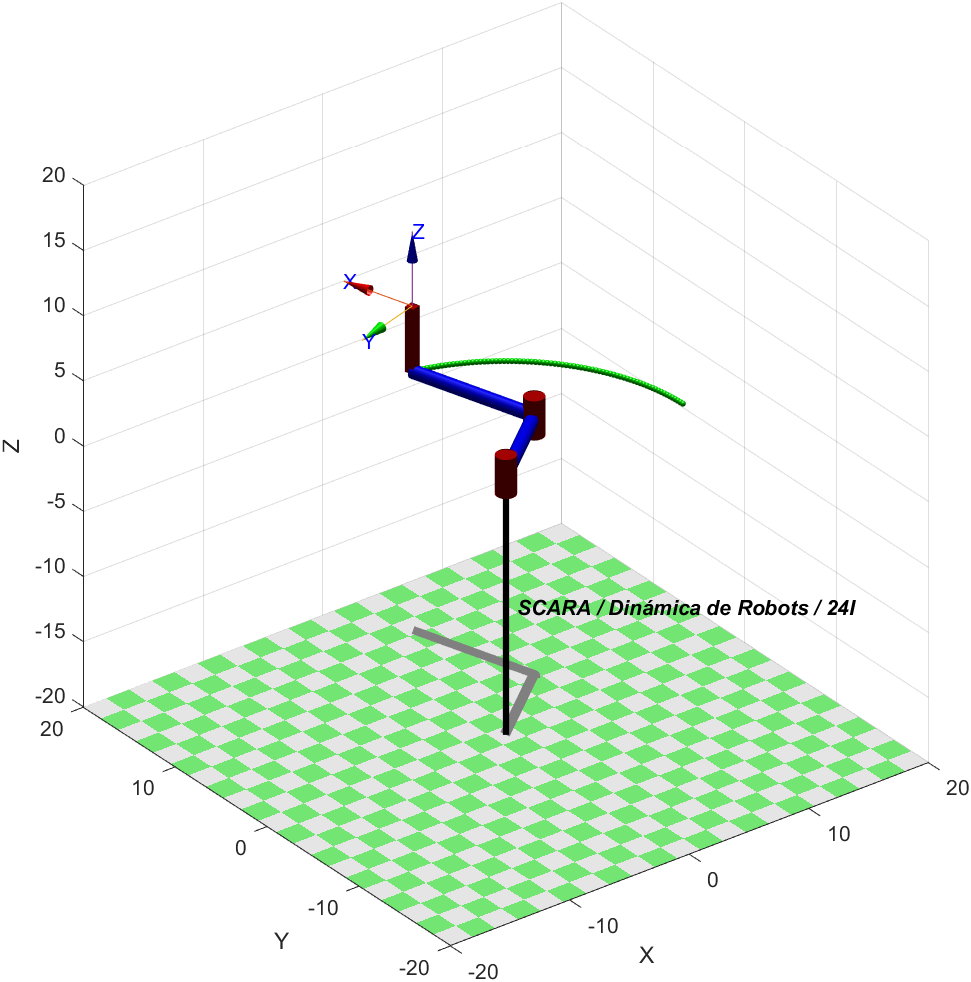
\includegraphics[width=0.5\textwidth]{G1.png}
\caption{Ilustración No. 2 de la Simulación.}
\label{fig:my_label}
\end{figure}

\begin{figure}[h!]
\centering
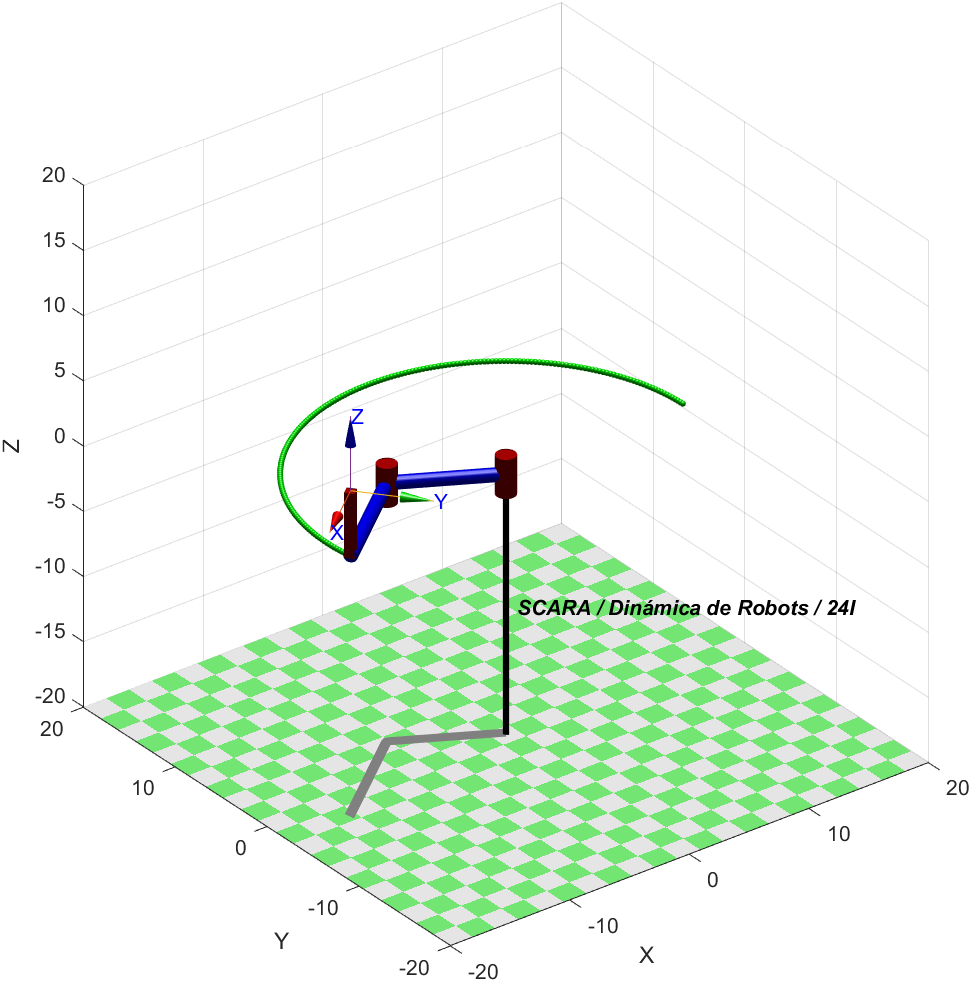
\includegraphics[width=0.5\textwidth]{G2.png}
\caption{Ilustración No. 3 de la Simulación.}
\label{fig:my_label}
\end{figure}

\begin{figure}[h!]
\centering
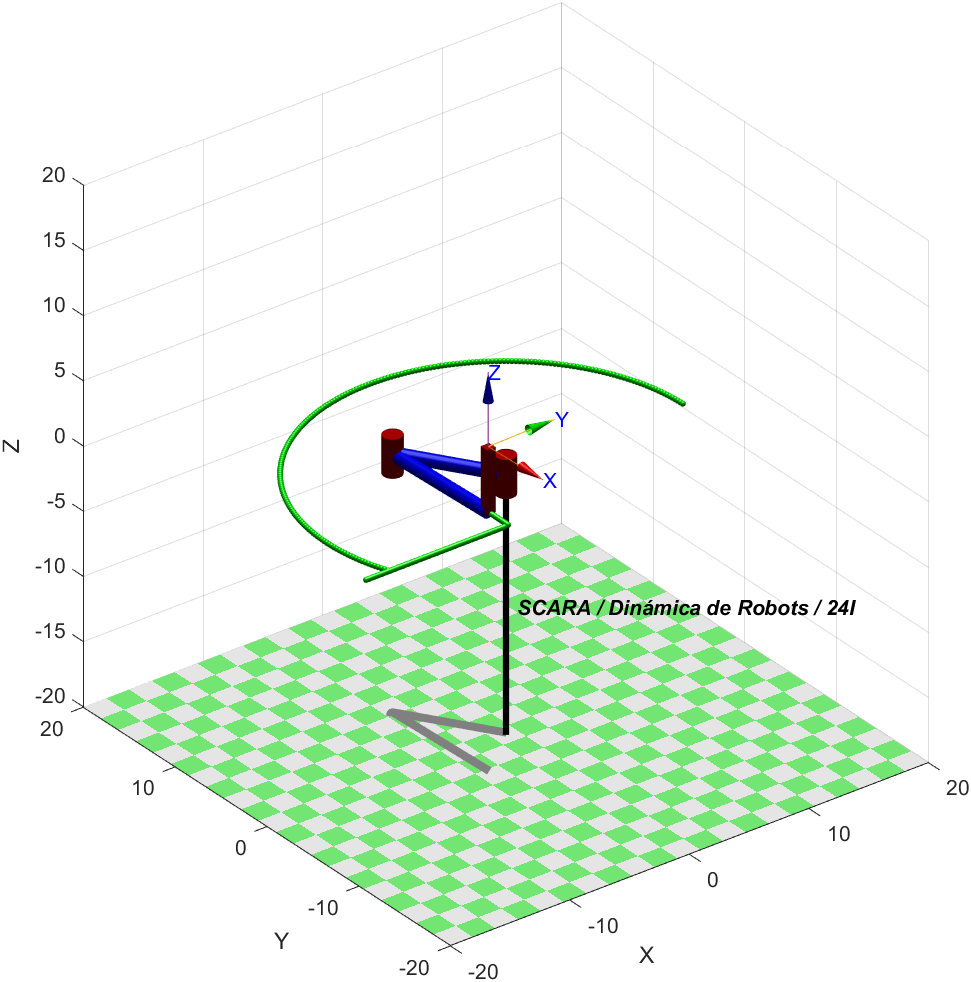
\includegraphics[width=0.5\textwidth]{G3.png}
\caption{Ilustración No. 4 de la Simulación.}
\label{fig:my_label}
\end{figure}

\begin{figure}[h!]
\centering
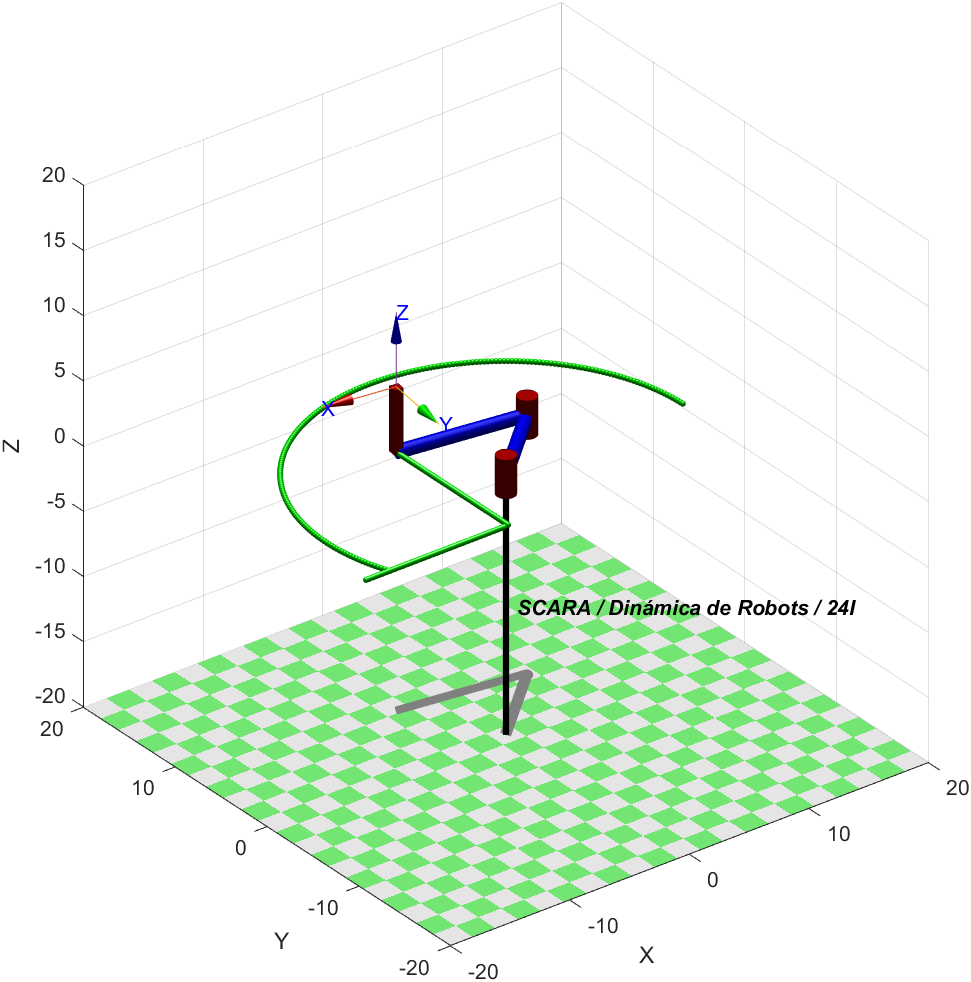
\includegraphics[width=0.4\textwidth]{G4.png}
\caption{Ilustración No. 5 de la Simulación.}
\label{fig:my_label}
\end{figure}

\begin{figure}[h!]
\centering
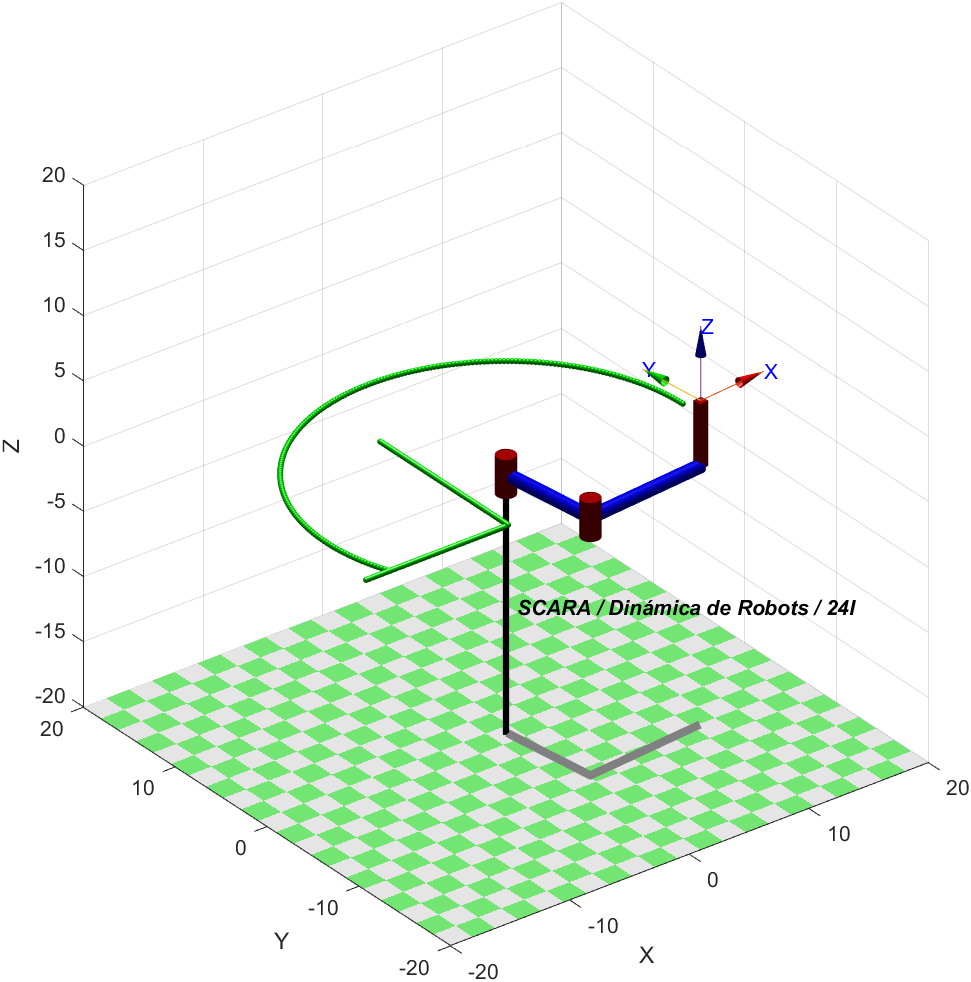
\includegraphics[width=0.4\textwidth]{G5.png}
\caption{Ilustración No. 6 de la Simulación.}
\label{fig:my_label}
\end{figure}

\begin{figure}[h!]
\centering
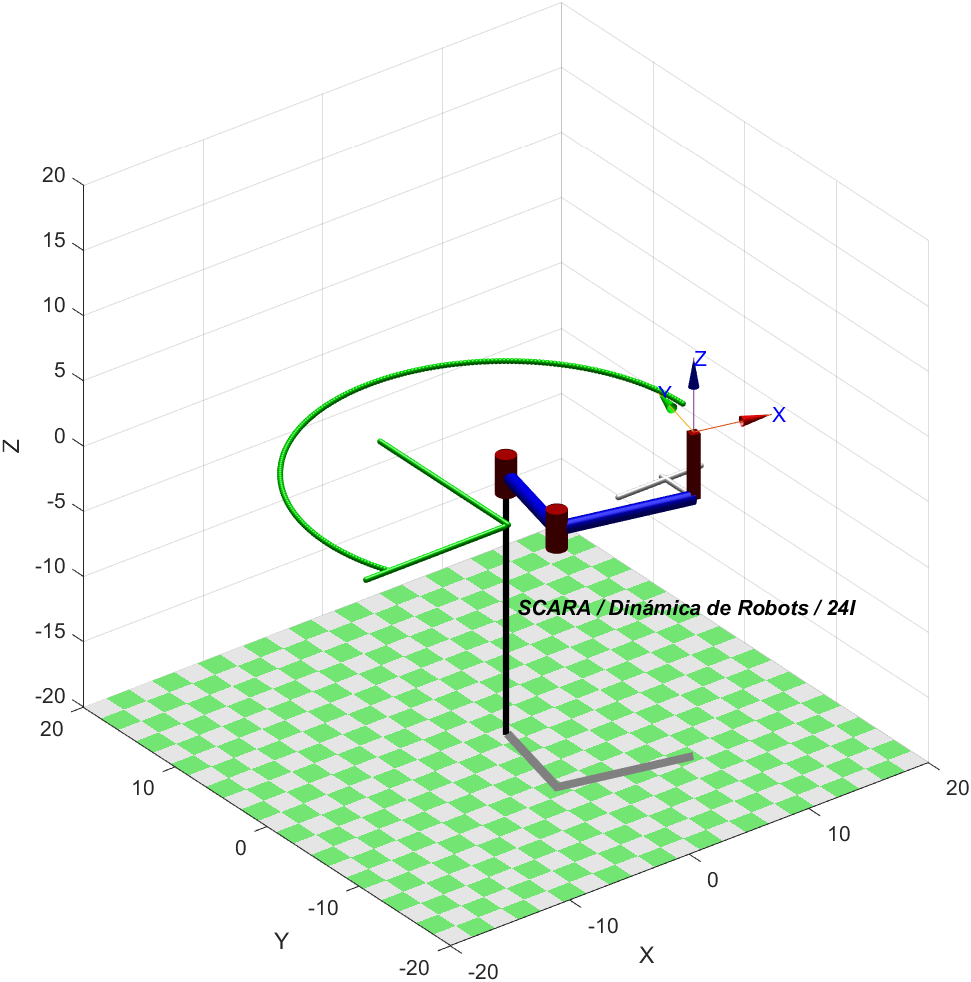
\includegraphics[width=0.4\textwidth]{GH0.png}
\caption{Ilustración No. 7 de la Simulación.}
\label{fig:my_label}
\end{figure}

\begin{figure}[h!]
\centering
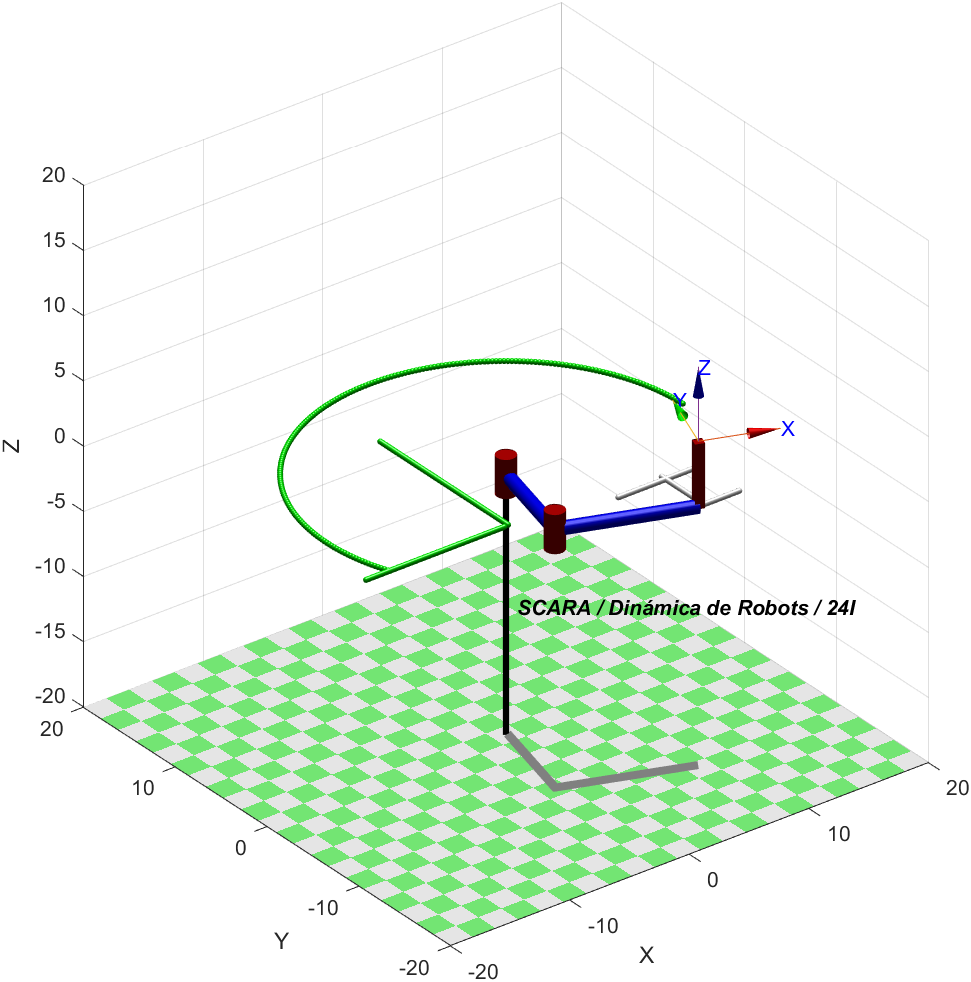
\includegraphics[width=0.4\textwidth]{GH1.png}
\caption{Ilustración No. 8 de la Simulación.}
\label{fig:my_label}
\end{figure}

\begin{figure}[h!]
\centering
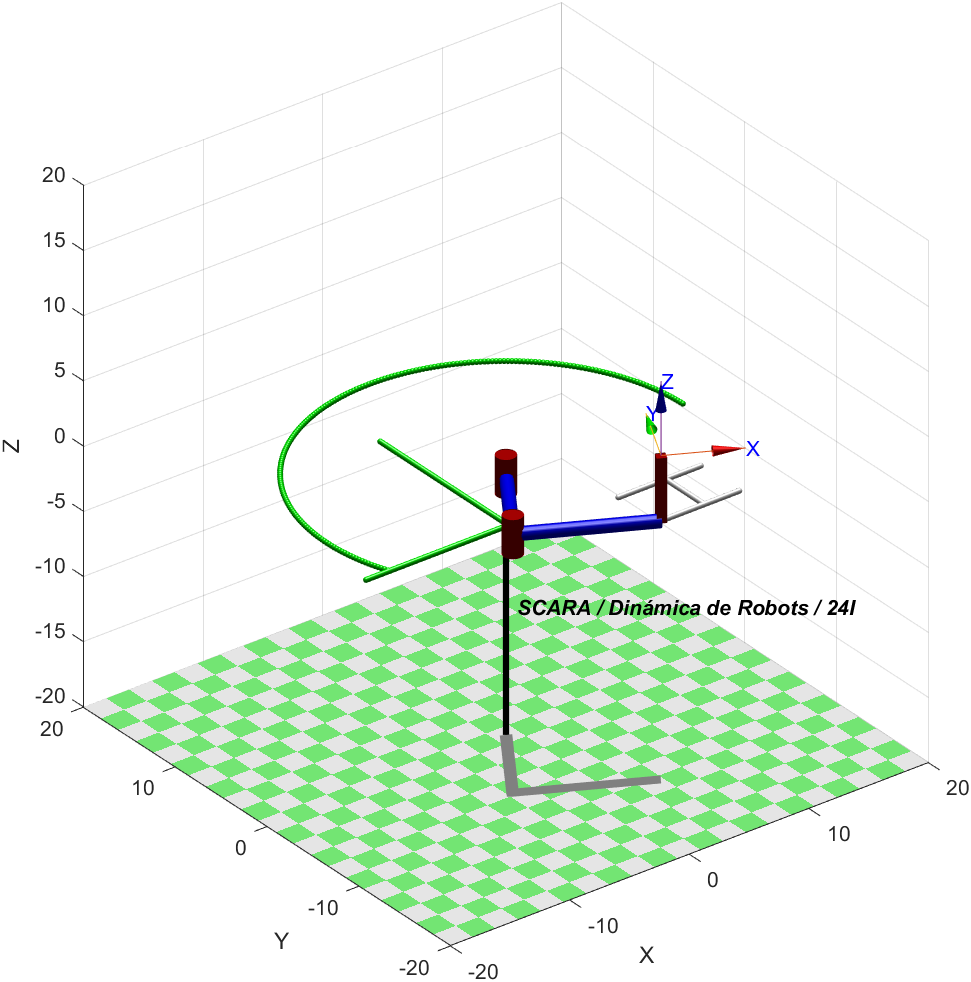
\includegraphics[width=0.4\textwidth]{GH2.png}
\caption{Ilustración No. 9 de la Simulación.}
\label{fig:my_label}
\end{figure}

\begin{figure}[h!]
\centering
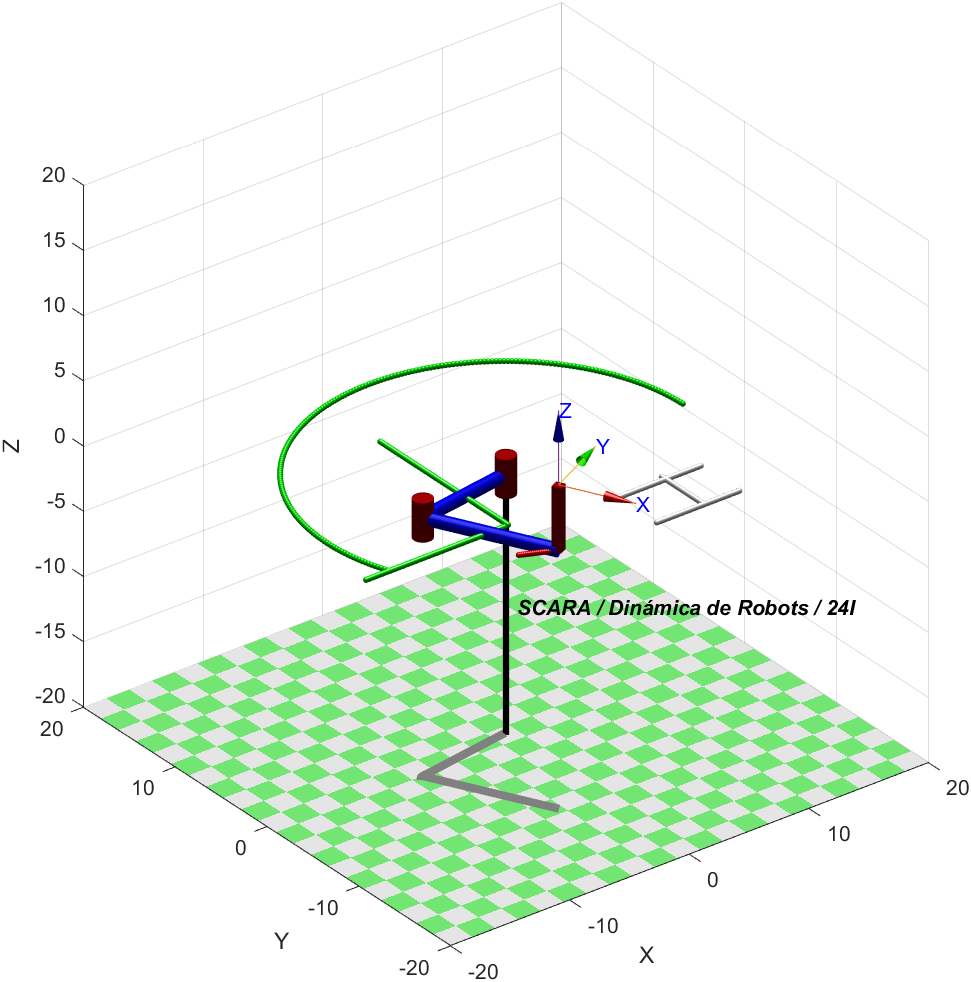
\includegraphics[width=0.4\textwidth]{GHA0.png}
\caption{Ilustración No. 10 de la Simulación.}
\label{fig:my_label}
\end{figure}

\begin{figure}[h!]
\centering
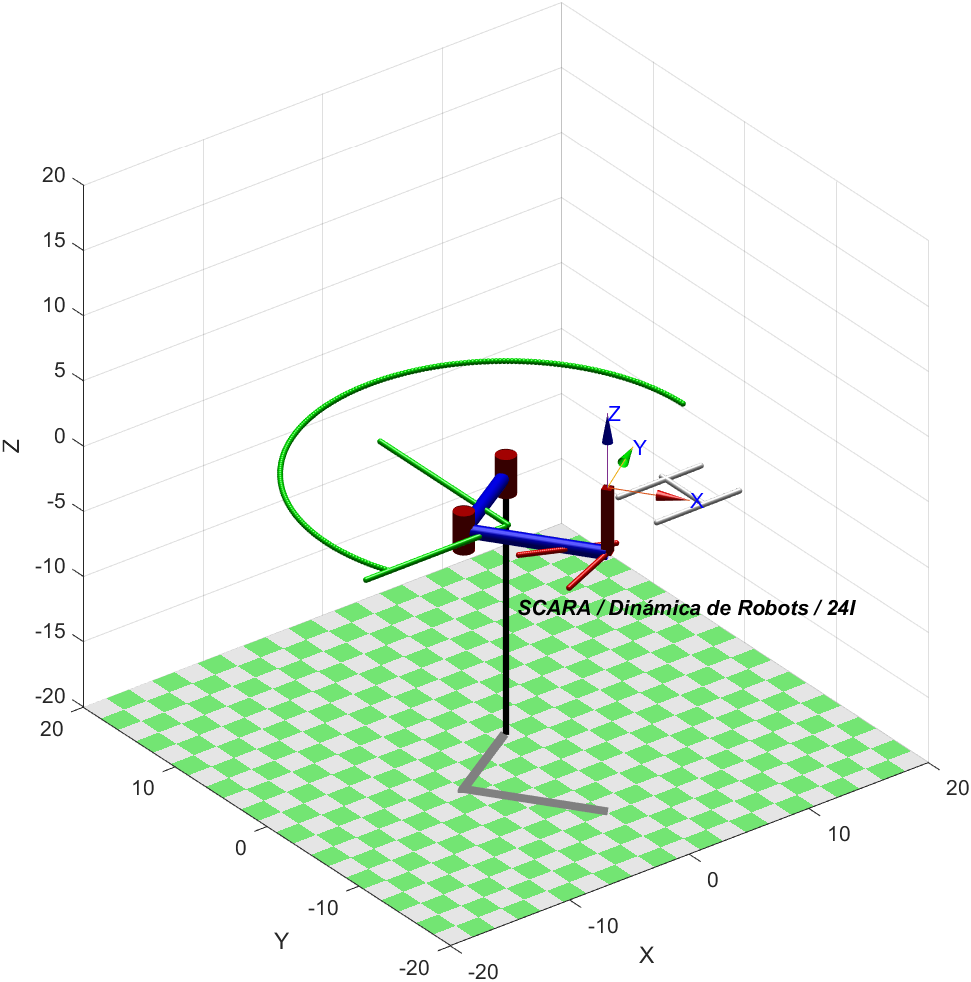
\includegraphics[width=0.4\textwidth]{GHA1.png}
\caption{Ilustración No. 11 de la Simulación.}
\label{fig:my_label}
\end{figure}

\begin{figure}[h!]
\centering
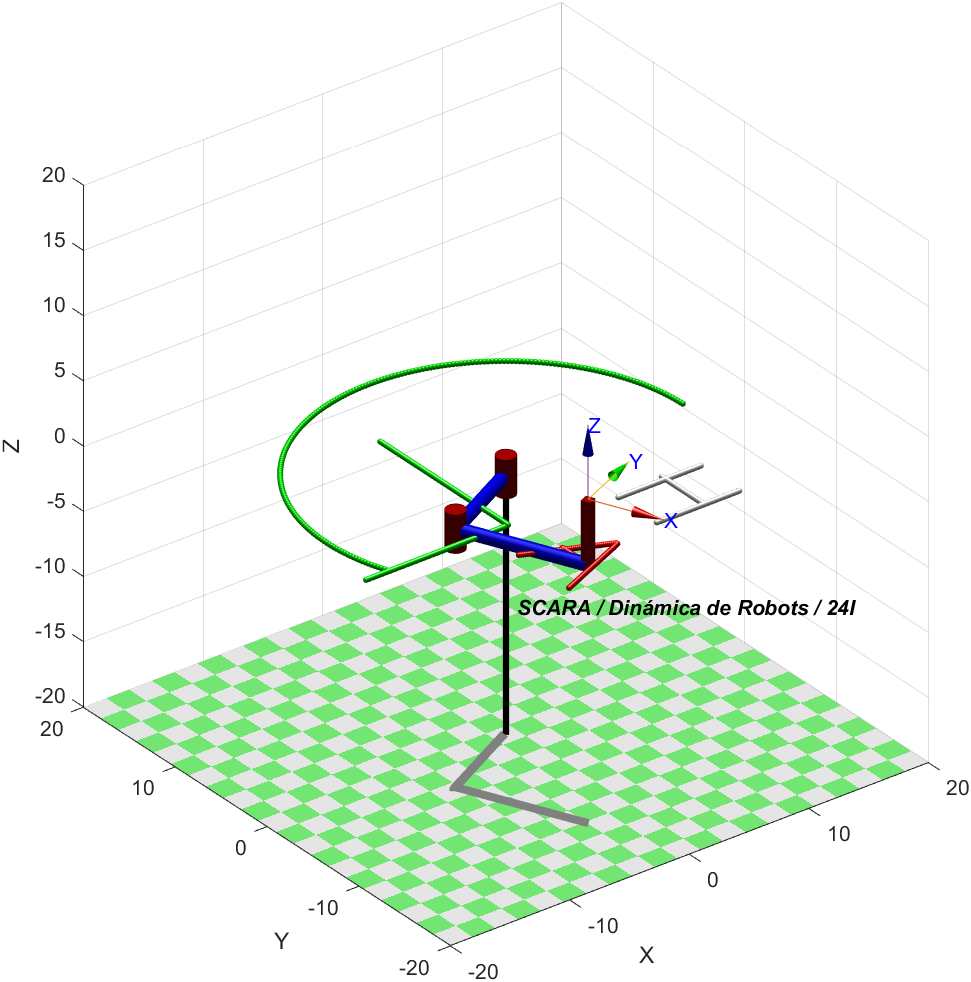
\includegraphics[width=0.4\textwidth]{GHA2.png}
\caption{Ilustración No. 12 de la Simulación.}
\label{fig:my_label}
\end{figure}

\begin{figure}[h!]
\centering
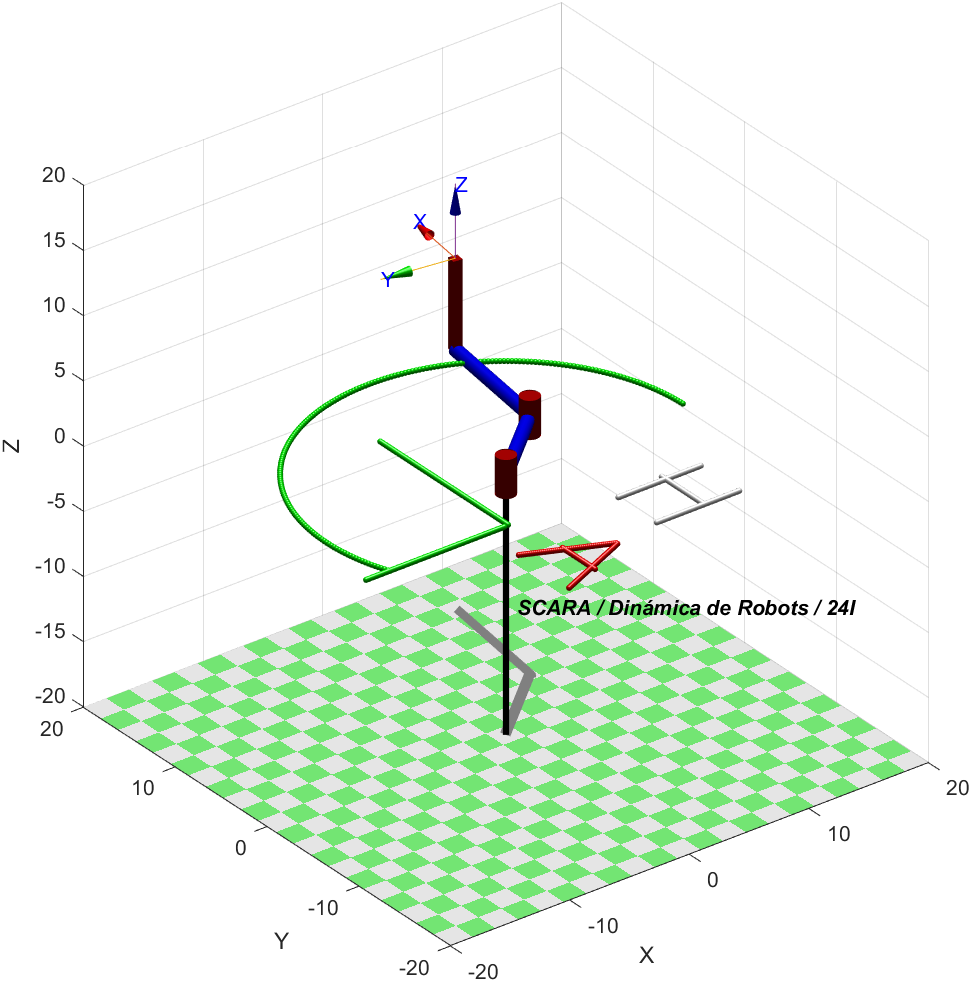
\includegraphics[width=0.45\textwidth]{GHA3.png}
\caption{Ilustración No. 13 de la Simulación.}
\label{fig:my_label}
\end{figure}

\begin{figure}[h!]
\centering
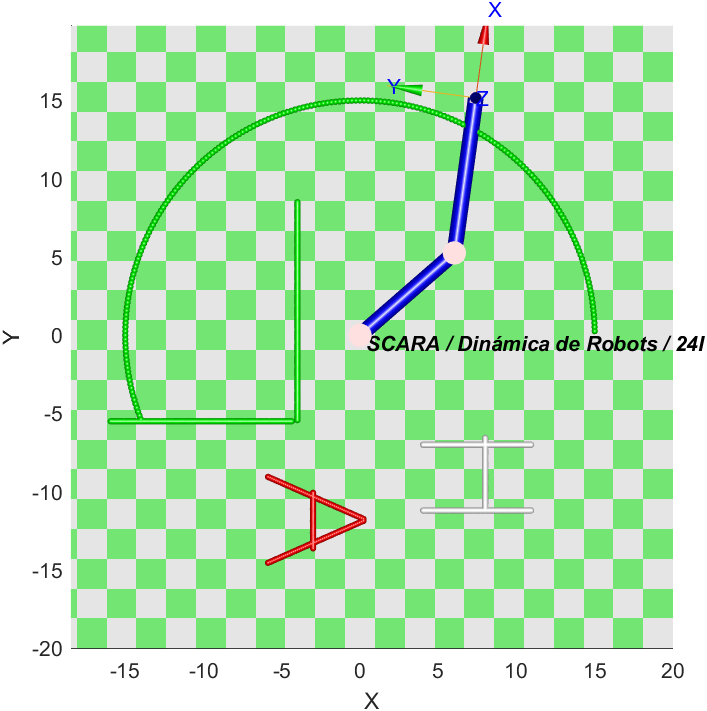
\includegraphics[width=0.45\textwidth]{GHA4.png}
\caption{Ilustración No. 14 de la Simulación.}
\label{fig:my_label}
\end{figure}

\begin{figure}[h!]
\centering
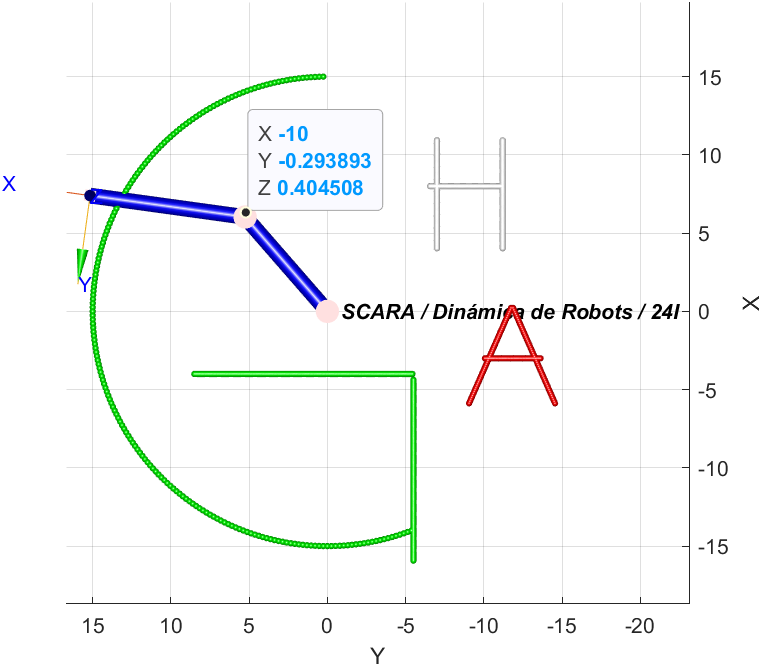
\includegraphics[width=0.45\textwidth]{GHA5.png}
\caption{Ilustración No. 15 de la Simulación.}
\label{fig:my_label}
\end{figure}

\begin{figure}[h!]
\centering
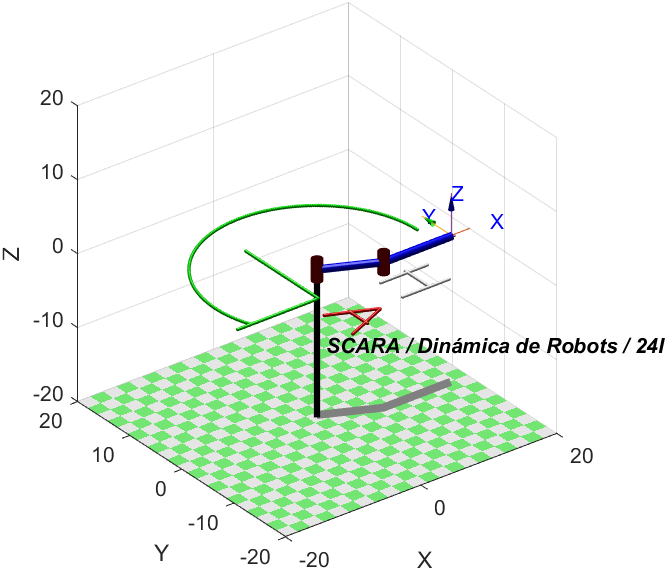
\includegraphics[width=0.45\textwidth]{GHAF.png}
\caption{Ilustración No. 16 de la Simulación.}
\label{fig:my_label}
\end{figure}

\begin{lstlisting}[language=Matlab]
% Limpiar todas las variables, consola y objetos de graficas
clear;
clc;
cla;

% Definicion de los eslabones del robot SCARA
L1 = Link([0 0 8 0 0]);  % Eslabon 1: rotativo, longitud 8
L2 = Link([0 0 10 0 0]); % Eslabon 2: rotativo, longitud 10
L3 = Link([0 0 0 0 1]);  % Eslabon 3: prismatico (a lo largo de Z, no usado aqui)

% Crear el robot SCARA
global R;  % Declara R como una variable global
R = SerialLink([L1, L2, L3], 'name', 'SCARA / Dinamica de Robots / 24I');

% Espacio de trabajo para visualizacion
global workSpaceLimits;  % Declara workSpaceLimits como una variable global
workSpaceLimits = [-20 20 -20 20 -20 20];

% Posicion inicial del robot
global h;  % Declara h como una variable global
if isempty(h) || ~isvalid(h)  % Si la figura no existe o no es valida
    h = figure;  % Crea una nueva figura y guarda su identificador
end
figure(h);  % Establece la figura del robot como la figura actual
R.plot([6, 8, 0],'workspace', workSpaceLimits);


% Longitudes de los eslabones, usadas en la cinematica inversa
l1 = 8;  % Longitud del primer eslabon
l2 = 10; % Longitud del segundo eslabon

tf = 20;    % Tiempo final
ts = 0.1;   % Paso de tiempo
t = 0:ts:tf;    % Vector de tiempo
N = length(t); % Numero de puntos en el vector de tiempo
%G %%
hx = zeros(1,N+1);  % Vector de coordenadas x del efector final
hy = zeros(1,N+1);  % Vector de coordenadas y del efector final
hz = zeros(1,N+1);  % Vector de coordenadas z del efector final

M = round(N);  % Limite maximo del primer segmento del dibujo

%% Calcula las posiciones articulares / Primer segmento
for k=1:M
    hx(k) = 15*cosd(k);   % Coordenada x del efector final -4 + 
    hy(k) = 15*sind(k);   % Coordenada y del efector final 7 + 
    hz(k) = 0;
    %pause(0.01); % Pausa breve para visualizar la animacion
    A = hx(k);
    B = hy(k);
end

% Dibuja la trayectoria
hold on;
for i = 1:N
    i;
    % Usar la funcion 'inverse_kinematics' para convertir puntos XY a angulos de junta
    [q1, q2] = inverse_kinematics(hx(i), hy(i), l1, l2); 
    % plot3(hx, hy, hz, 'r.');
    p = [hx(i), hy(i), hz(i)]; % Obtiene el punto actual de la trayectoria
    plot_sphere(p, 0.2, 'g'); % Dibuja una esfera en el punto actual para visualizar la trayectoria

    R.plot([q1 q2 5],'workspace', workSpaceLimits); % Tercer valor corresponde a d3 que es cero
    drawnow;

end

% *Linea de izquierda a derecha (color verde)*
hx_der = zeros(1,N+1);  % Vector de coordenadas x del efector final (derecha a izquierda)
hy_der = zeros(1,N+1);  % Vector de coordenadas y del efector final
hz_der = zeros(1,N+1);  % Vector de coordenadas z del efector final

for i = 1:N
    hx_der(i) = -16 + (14/N) * i;   % Coordenada x del efector final (derecha a izquierda)
    hy_der(i) = -5.5;               % Coordenada y constante para una linea recta
    hz_der(i) = 0;
end

% Dibuja la trayectoria (derecha a izquierda)
hold on;
for i = 1:(N/1.2)
    [q1_der, q2_der] = inverse_kinematics(hx_der(i), hy_der(i), l1, l2); 
    p_der = [hx_der(i), hy_der(i), hz_der(i)]; % Obtiene el punto actual de la trayectoria
    plot_sphere(p_der, 0.2, 'g'); % Dibuja una esfera en el punto actual para visualizar la trayectoria (color verde)
    R.plot([q1_der q2_der 5],'workspace', workSpaceLimits); % Color verde
    drawnow;
end

% *Linea de abajo a arriba (color verde)*
hx_der = zeros(1,N+1);  % Vector de coordenadas x del efector final
hy_der = zeros(1,N+1);  % Vector de coordenadas y del efector final
hz_der = zeros(1,N+1);  % Vector de coordenadas z del efector final

for i = 1:N
    hx_der(i) = -4;   % Coordenada x del efector final
    hy_der(i) = -5.5 + (14/N) * i;               % Coordenada y
    hz_der(i) = 0;
end

% Dibuja la trayectoria (de abajo a arriba)
hold on;
for i = 1:N
    [q1_der, q2_der] = inverse_kinematics(hx_der(i), hy_der(i), l1, l2); 
    p_der = [hx_der(i), hy_der(i), hz_der(i)]; % Obtiene el punto actual de la trayectoria
    plot_sphere(p_der, 0.2, 'g'); % Dibuja una esfera en el punto actual para visualizar la trayectoria (color verde)
    R.plot([q1_der q2_der 5],'workspace', workSpaceLimits); % Color verde
    drawnow;
end

% H %%
% *Linea de izquierda a derecha (color blanco)*
hx_izq = zeros(1,N+1);  % Vector de coordenadas x del efector final (izquierda a derecha)
hy_izq = zeros(1,N+1);  % Vector de coordenadas y del efector final
hz_izq = zeros(1,N+1);  % Vector de coordenadas z del efector final

for i = 1:N
    hx_izq(i) = -3 + (14/N) * (N-i);   % Coordenada x del efector final (izquierda a derecha)
    hy_izq(i) = -7;               % Coordenada y constante para una linea recta
    hz_izq(i) = 0;
end

% Dibuja la trayectoria (izquierda a derecha)
hold on;
for i = 1:(N/2)
    [q1_izq, q2_izq] = inverse_kinematics(hx_izq(i), hy_izq(i), l1, l2); 
    p_izq = [hx_izq(i), hy_izq(i), hz_izq(i)]; % Obtiene el punto actual de la trayectoria
    plot_sphere(p_izq, 0.2, 'w'); % Dibuja una esfera en el punto actual para visualizar la trayectoria (color blanco)
    R.plot([q1_izq q2_izq 5],'workspace', workSpaceLimits); % Color blanco
    drawnow;
end

% *Linea de abajo a arriba (color blanco)*
hx_der = zeros(1,N+1);  % Vector de coordenadas x del efector final
hy_der = zeros(1,N+1);  % Vector de coordenadas y del efector final
hz_der = zeros(1,N+1);  % Vector de coordenadas z del efector final

for i = 1:N
    hx_der(i) = 8;   % Coordenada x del efector final
    hy_der(i) = -6.5 - (14/N) * i;               % Coordenada y
    hz_der(i) = 0;
end

% Dibuja la trayectoria (de abajo a arriba)
hold on;
for i = 1:(N/3)
    [q1_der, q2_der] = inverse_kinematics(hx_der(i), hy_der(i), l1, l2); 
    p_der = [hx_der(i), hy_der(i), hz_der(i)]; % Obtiene el punto actual de la trayectoria
    plot_sphere(p_der, 0.2, 'w'); % Dibuja una esfera en el punto actual para visualizar la trayectoria (color blanco)
    R.plot([q1_der q2_der 5],'workspace', workSpaceLimits); % Color blanco
    drawnow;
end

% *Linea de derecha a izquierda (color blanco)*
hx_der = zeros(1,N+1);  % Vector de coordenadas x del efector final (derecha a izquierda)
hy_der = zeros(1,N+1);  % Vector de coordenadas y del efector final
hz_der = zeros(1,N+1);  % Vector de coordenadas z del efector final

for i = 1:N
    hx_der(i) = -3 + (14/N) * (N-i);   % Coordenada x del efector final (derecha a izquierda)
    hy_der(i) = -11.2;               % Coordenada y constante para una linea recta
    hz_der(i) = 0;
end

% Dibuja la trayectoria (derecha a izquierda)
hold on;
for i = 1:(N/2)
    [q1_der, q2_der] = inverse_kinematics(hx_der(i), hy_der(i), l1, l2); 
    p_der = [hx_der(i), hy_der(i), hz_der(i)]; % Obtiene el punto actual de la trayectoria
    plot_sphere(p_der, 0.2, 'w'); % Dibuja una esfera en el punto actual para visualizar la trayectoria (color blanco)
    R.plot([q1_der q2_der 5],'workspace', workSpaceLimits); % Color blanco
    drawnow;
end
% A %%
% *Linea de derecha a izquierda diagonal hacia abajo*
hx_der = zeros(1,N+1);  % Vector de coordenadas x del efector final (derecha a izquierda)
hy_der = zeros(1,N+1);  % Vector de coordenadas y del efector final
hz_der = zeros(1,N+1);  % Vector de coordenadas z del efector final

for i = 1:N
    hx_der(i) = -6 + (25/N) * i;   % Coordenada x del efector final (derecha a izquierda)
    hy_der(i) = -9 - (11/N) * i;               % Coordenada y constante para una linea recta (-8)
    hz_der(i) = 0;
end

% Dibuja la trayectoria (derecha a izquierda)
hold on;
for i = 1:(N/4)
    [q1_der, q2_der] = inverse_kinematics(hx_der(i), hy_der(i), l1, l2); 
    p_der = [hx_der(i), hy_der(i), hz_der(i)]; % Obtiene el punto actual de la trayectoria
    plot_sphere(p_der, 0.2, 'r'); % Dibuja una esfera en el punto actual para visualizar la trayectoria (color rojo)
    R.plot([q1_der q2_der 5],'workspace', workSpaceLimits); % Color rojo
    drawnow;
end

% *Linea de derecha a izquierda diagonal hacia arriba (color rojo)*
hx_der = zeros(1,N+1);  % Vector de coordenadas x del efector final (derecha a izquierda)
hy_der = zeros(1,N+1);  % Vector de coordenadas y del efector final
hz_der = zeros(1,N+1);  % Vector de coordenadas z del efector final

for i = 1:N
    hx_der(i) = -6 + (25/N) * i;   % Coordenada x del efector final (derecha a izquierda)
    hy_der(i) = -14.6 + (11/N) * i;               % Coordenada y constante para una linea recta (-8)
    hz_der(i) = 0;
end

% Dibuja la trayectoria (derecha a izquierda) 
hold on;
for i = 1:(N/4)
    [q1_der, q2_der] = inverse_kinematics(hx_der(i), hy_der(i), l1, l2); 
    p_der = [hx_der(i), hy_der(i), hz_der(i)]; % Obtiene el punto actual de la trayectoria
    plot_sphere(p_der, 0.2, 'r'); % Dibuja una esfera en el punto actual para visualizar la trayectoria (color rojo)
    R.plot([q1_der q2_der 5],'workspace', workSpaceLimits); % Color rojo
    drawnow;
end

% *Linea de abajo a arriba (color rojo)*
hx_der = zeros(1,N+1);  % Vector de coordenadas x del efector final
hy_der = zeros(1,N+1);  % Vector de coordenadas y del efector final
hz_der = zeros(1,N+1);  % Vector de coordenadas z del efector final

for i = 1:N
    hx_der(i) = -3;   % Coordenada x del efector final
    hy_der(i) = -10 - (14/N) * i;               % Coordenada y
    hz_der(i) = 0;
end

% Dibuja la trayectoria (de abajo a arriba)
hold on;
for i = 1:(N/3.8)
    [q1_der, q2_der] = inverse_kinematics(hx_der(i), hy_der(i), l1, l2); 
    p_der = [hx_der(i), hy_der(i), hz_der(i)]; % Obtiene el punto actual de la trayectoria
    plot_sphere(p_der, 0.2, 'r'); % Dibuja una esfera en el punto actual para visualizar la trayectoria (color rojo)
    R.plot([q1_der q2_der 5],'workspace', workSpaceLimits); % Color rojo
    drawnow;
end

hold off;

% Crear los campos de texto para q1 y q2
global q1_text q2_text;
q1_text = uicontrol('Style', 'edit', 'Position', [20 60 100 20], 'String', '0');
q2_text = uicontrol('Style', 'edit', 'Position', [20 30 100 20], 'String', '0');

% Crear un boton para actualizar la posicion del robot
update_button = uicontrol('Style', 'pushbutton', 'Position', [20 90 100 20], 'String', 'Actualizar');

% Definir la funcion de callback para el boton
set(update_button, 'Callback', @updateRobot);

% Funcion de callback para actualizar la posicion del robot
function updateRobot(src, event)
    % Obtener los campos de texto de la figura
    global q1_text q2_text R workSpaceLimits h;  % Agregar workSpaceLimits y h a la lista de variables globales
    q1 = str2double(get(q1_text, 'String')) * (pi / 180);
    q2 = str2double(get(q2_text, 'String')) * (pi / 180);
    z = 0.1;

    % Borrar el robot anterior
    robot_graphics = findobj(h, 'Type', 'Patch');  % Encuentra los objetos graficos que representan al robot
    delete(robot_graphics);  % Borra solo el robot, no toda la figura

    % Dibujar el robot con los nuevos valores de q1 y q2
    R.plot([q1, q2, z],'workspace', workSpaceLimits);
end

% Funcion de cinematica inversa
function [q1, q2] = inverse_kinematics(x, y, L1, L2)
    % Calcula theta2
    c2 = (x^2 + y^2 - L1^2 - L2^2) / (2 * L1 * L2);

    if c2 < -1 || c2 > 1
        error('El punto [%f, %f] esta fuera del alcance del robot.', x, y);
    end
    theta2 = acos(c2);  % Solucion principal

    % Calcula theta1
    k1 = L1 + L2 * cos(theta2);
    k2 = L2 * sin(theta2);
    theta1 = atan2(y, x) - atan2(k2, k1);

    % Asigna resultados a las variables de salida
    q1 = theta1;
    q2 = theta2;
end
\end{lstlisting}

\section{VI. Solución con IoT y Cinemática Inversa para Manipular un Robot SCARA Real}

\begin{figure}[h!]
\centering
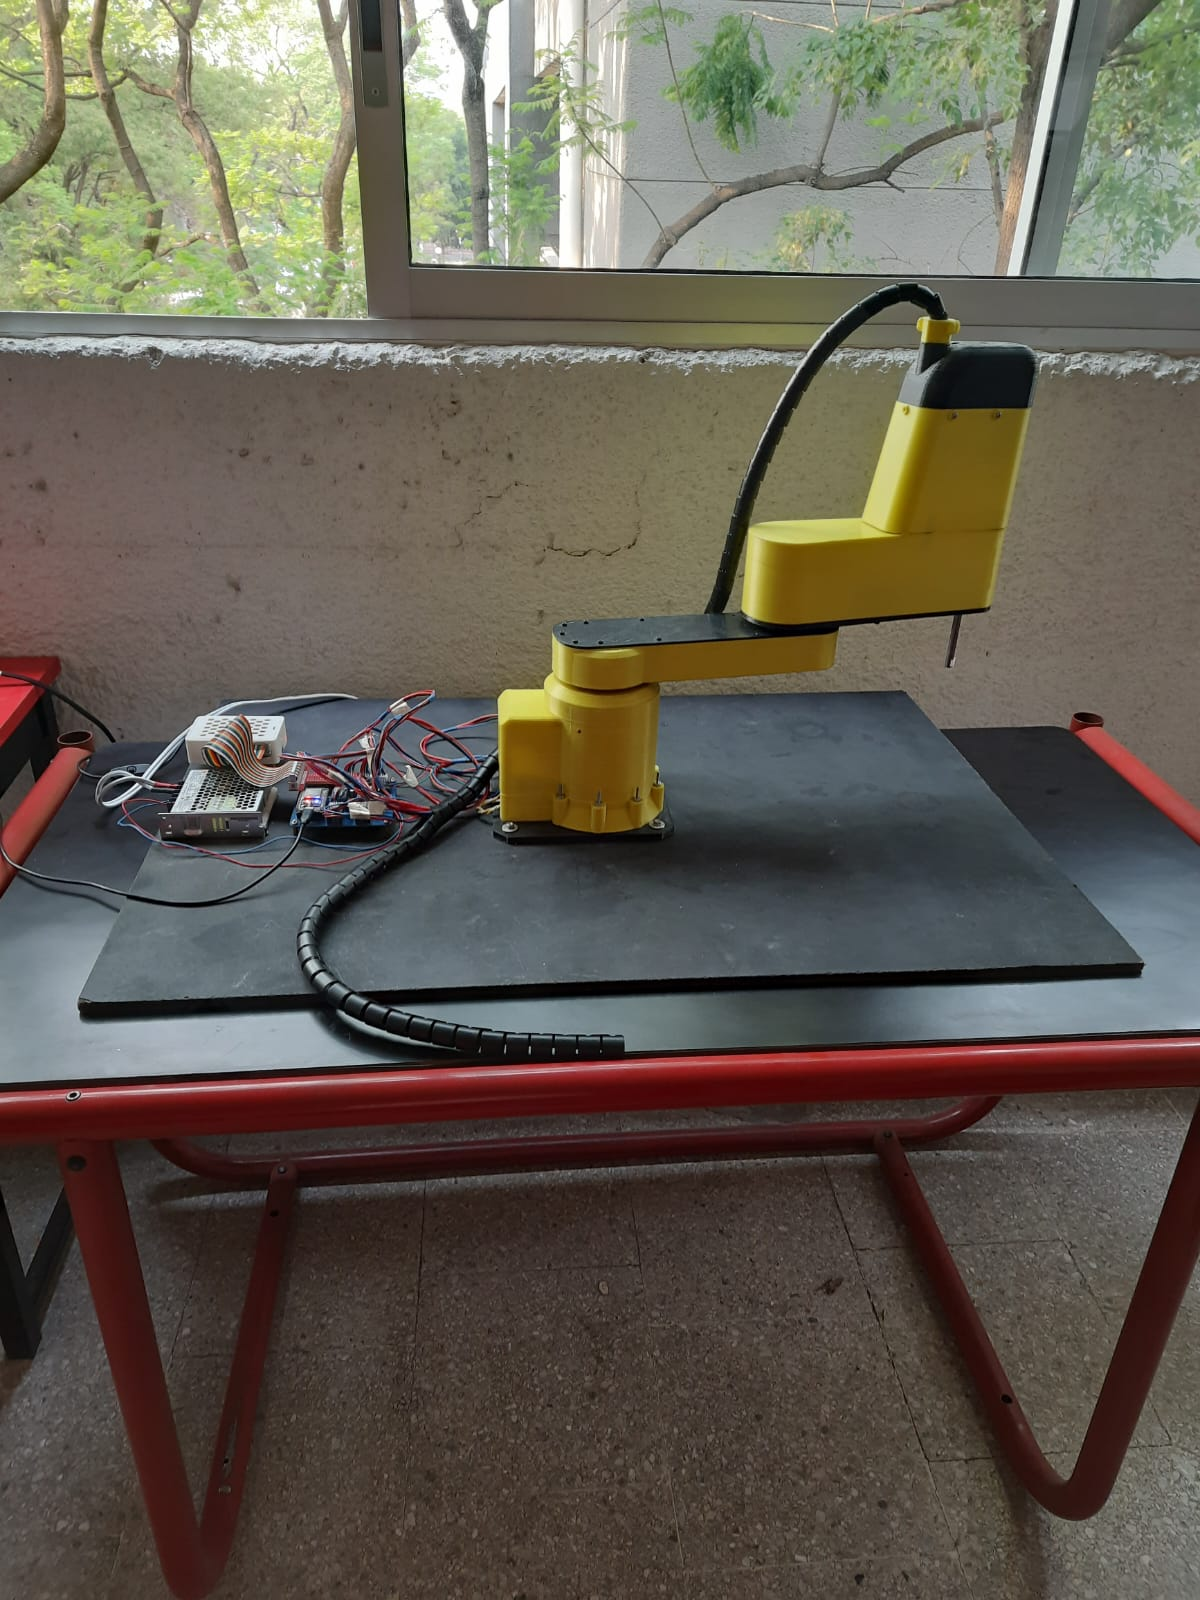
\includegraphics[width=0.45\textwidth]{SCARA1.jpg}
\caption{Robot SCARA del Laboratorio de desarrollo de proyectos mecatrónicos y electrónicos.}
\label{fig:my_label}
\end{figure}

La Universidad Autónoma Metropolitana (UAM) Azcapotzalco, a través del "Laboratorio de desarrollo de proyectos mecatrónicos y electrónicos", nos brindó la oportunidad de trabajar con un robot SCARA real para poner en práctica los conceptos de control robótico y simulación aprendidos en la UEA de Dinámica de Robots que se imparte en esta unidad por el profesor Mtro. Jorge Miguel Jaimes Ponce. 


El laboratorio cuenta con instalaciones de vanguardia y personal altamente calificado para el desarrollo de proyectos en robótica, automatización y control de sistemas y el profesor se destaca por su enfoque en la robótica y la mecatrónica, ofreciendo proyectos de investigación en estas áreas.

La UAM Azcapotzalco, reconocida por su excelencia académica y su compromiso con la innovación tecnológica, nos brindó la oportunidad de utilizar su robot SCARA para poner en práctica el control mediante cinemática inversa.

\subsection{I. SIMULACIÓN EN MATLAB:}

\subsubsection{Adaptación del modelo del robot}

El modelo del robot SCARA en MATLAB Robotics Toolbox se adaptó cuidadosamente a las características del robot real proporcionado por la UAM Azcapotzalco. Esto incluyó la medición precisa de parámetros como las longitudes de los eslabones, los ángulos de rotación y los límites de movimiento.

\subsubsection{Implementación de cinemática inversa}
Se implementó un algoritmo de cinemática inversa para calcular las posiciones angulares de las articulaciones del robot a partir de coordenadas deseadas en el espacio. El algoritmo se basó en el la libreria de Peter Corke que a su vez se basa en el método de Denavit-Hartenberg y se ajustó para considerar las limitaciones específicas del robot real.

\subsubsection{Simulación de dibujo de letras}
Utilizando el modelo del robot y el algoritmo de cinemática inversa, se simuló el movimiento del robot dibujando las letras ``G'', ``H'' y ``A'' en el espacio. La simulación permitió visualizar las trayectorias de las letras y verificar el correcto funcionamiento del control.

\begin{lstlisting}[language=Matlab]
clc
clear
close all
%%%%%%%%%%%%%%%%%%%%%%%%%%%%%%%%%%%%%%%%%%%%%%%%%%%
% Parametros de conexion MQTT
topic = 'Matlab'; % Tema al que se publicara
mqttClient = mqttclient("mqtt://192.168.137.1:1883");% Direccion del broker MQTT

% Suscripcion al tema Matlab
try
    subscribe(mqttClient, topic);
    disp(['Suscrito al tema: ' topic]);
catch ME
    disp(['Error al suscribirse al tema: ' ME.message]);
    return;
end
% Fin de Parametros de conexion MQTT
%%%%%%%%%%%%%%%%%%%%%%%%%%%%%%%%%%%%%%%%%%%%%%%%%%%
% CONSTRUCCION Y SIMULACION CON ROBOTICS TOOLBOX
% Definir las articulaciones
L1 = Link('d', 158, 'a', 200, 'alpha', 0);
L2 = Link('d', 43, 'a', 200, 'alpha', 0);
L3 = Link('d', 52, 'a', 0, 'alpha', 0);

% Simulacion del robot SCARA con sus dimensiones
global R;
R = SerialLink([L1, L2, L3], 'name', 'SCARA / Dinamica de Robots / 24I');

% Espacio de trabajo para visualizacion
global workSpaceLimits;  % Declara workSpaceLimits como una variable global
workSpaceLimits = [-500 500 -500 500 -500 500];

% Posicion inicial del robot
global h;  % Declara h como una variable global
if isempty(h) || ~isvalid(h)  % Si la figura no existe o no es valida
    h = figure;  % Crea una nueva figura y guarda su identificador
end
figure(h);  % Establece la figura del robot como la figura actual
R.plot([0, 0, 0],'workspace', workSpaceLimits);
% FIN DE LA CONSTRUCCION Y SIMULACION CON ROBOTICS TOOLBOX
%%%%%%%%%%%%%%%%%%%%%%%%%%%%%%%%%%%%%%%%%%%%%%%%%%%
\end{lstlisting}

\begin{figure}[h!]
\centering
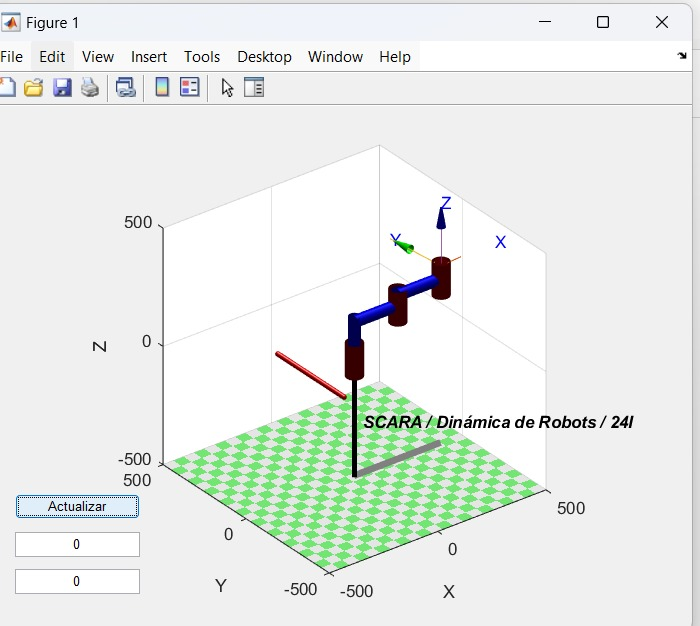
\includegraphics[width=0.45\textwidth]{SCARA0.jpg}
\caption{Simulación del Robot SCARA del Laboratorio de desarrollo de proyectos mecatrónicos y electrónicos.}
\label{fig:my_label}
\end{figure}

\begin{lstlisting}[language=Matlab]
% Longitudes de los eslabones, usadas en la cinematica inversa
l1 = L1.a;
l2 = L2.a;

tf = 20;    % Tiempo final
ts = 0.1;   % Paso de tiempo
t = 0:ts:tf;    % Vector de tiempo
N = length(t); % Numero de puntos en el vector de tiempo

% Linea de abajo a arriba
hx_der = zeros(1,N+1);  % Vector de coordenadas x del efector final
hy_der = zeros(1,N+1);  % Vector de coordenadas y del efector final
hz_der = zeros(1,N+1);  % Vector de coordenadas z del efector final

for i = 1:N
    hx_der(i) = -200;   % Coordenada x del efector final
    hy_der(i) = -200 + (400/N) * i;               % Coordenada y
    hz_der(i) = 0;
end

% Dibuja la trayectoria (de abajo a arriba)
hold on;
for i = 1:N
    [q1_der, q2_der] = inverse_kinematics(hx_der(i), hy_der(i), l1, l2); 

    % Resultados
    fprintf("q1 = %.11f\n", q1_der);
    fprintf("q2 = %.11f\n", q2_der);

    % Empaquetamiento datos en estructura JSON
    data = struct('q1', q1_der, 'q2', q2_der);
    jsonData = jsonencode(data);

    % Publicacion del mensaje JSON al tema
    message = jsonData;
    %write(mqttClient, topic, message);  % Descomentar esta linea para enviar el mensaje

    p_der = [hx_der(i), hy_der(i), hz_der(i)]; % Obtiene el punto actual de la trayectoria
    plot_sphere(p_der, 10, 'r'); % Dibuja una esfera en el punto actual para visualizar la trayectoria (color verde)
    R.plot([q1_der q2_der 0],'workspace', workSpaceLimits); % Color verde
    drawnow;
end
hold off;

% Funcion de cinematica inversa
function [q1, q2] = inverse_kinematics(x, y, L1, L2)
    % Calcula theta2
    c2 = (x^2 + y^2 - L1^2 - L2^2) / (2 * L1 * L2);

    if c2 < -1 || c2 > 1
        error('El punto [%f, %f] esta fuera del alcance del robot.', x, y);
    end
    theta2 = acos(c2);  % Solucion principal

    % Calcula theta1
    k1 = L1 + L2 * cos(theta2);
    k2 = L2 * sin(theta2);
    theta1 = atan2(y, x) - atan2(k2, k1);

    % Asigna resultados a las variables de salida
    q1 = theta1;
    q2 = theta2;
end
\end{lstlisting}

\begin{figure}[h!]
\centering
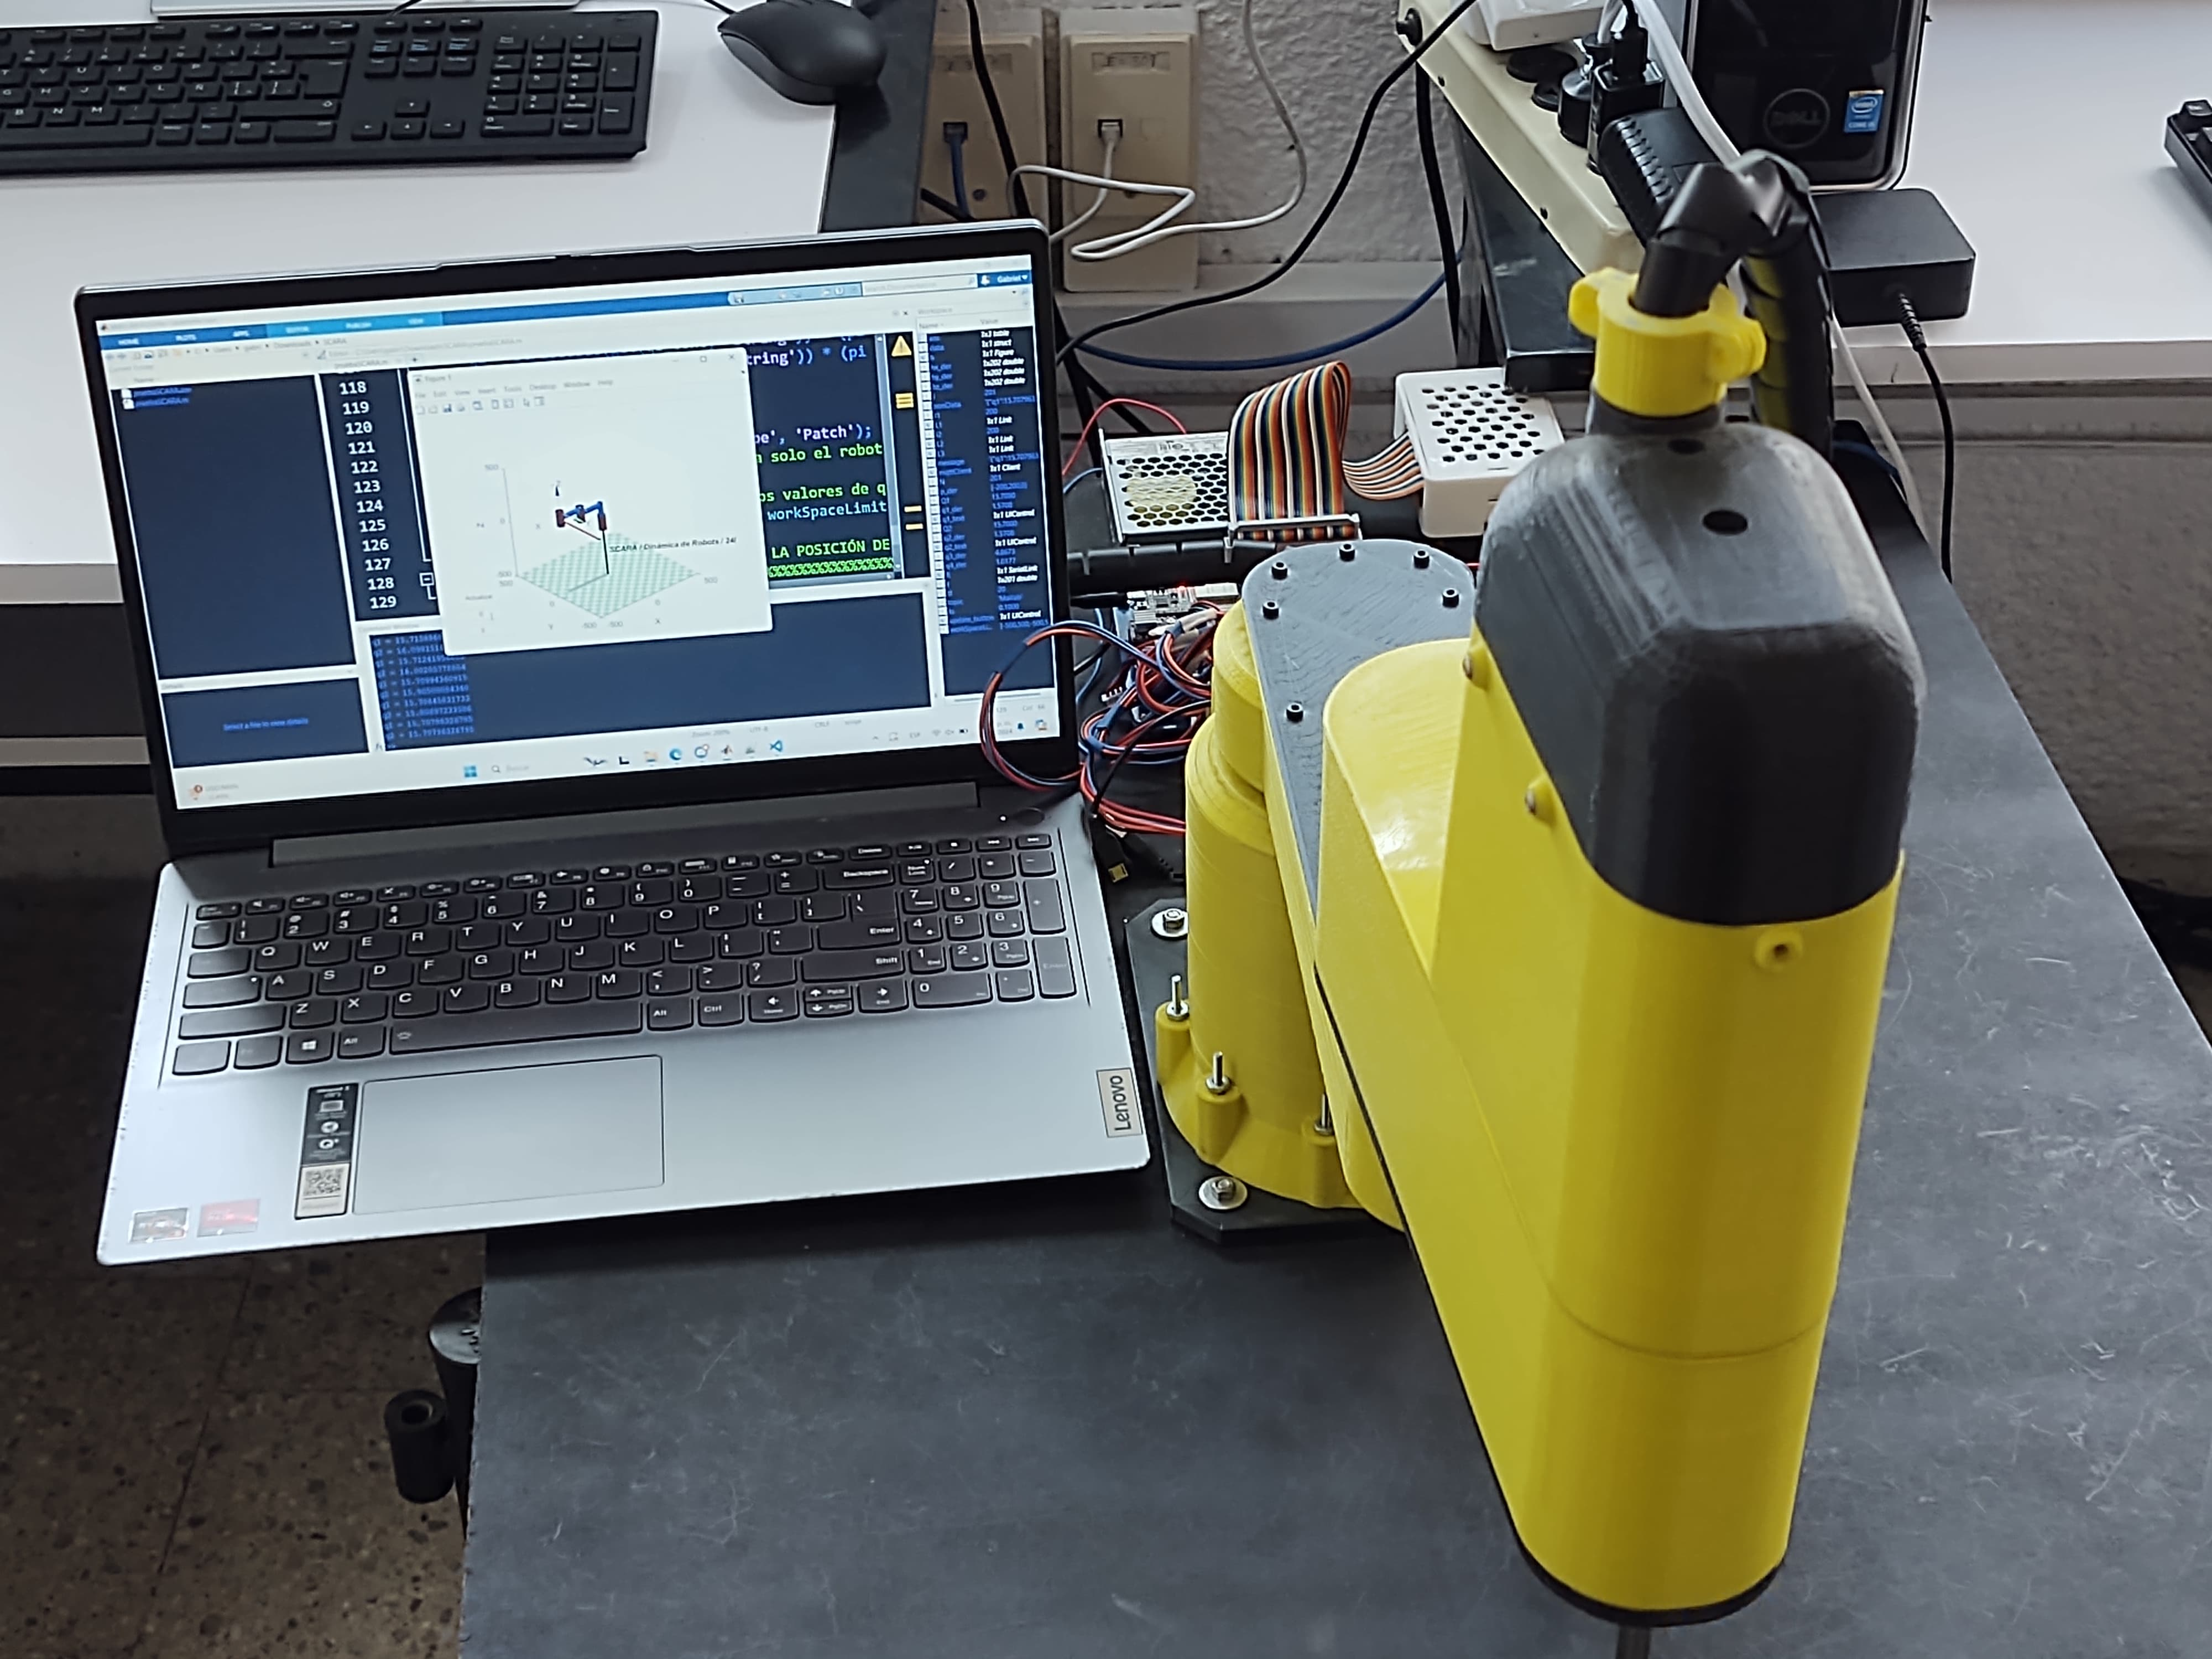
\includegraphics[width=0.45\textwidth]{SCARA2.jpg}
\caption{Pruebas del moviento del Robot}
\label{fig:my_label}
\end{figure}

\begin{lstlisting}[language=Matlab]
%%%%%%%%%%%%%%%%%%%%%%%%%%%%%%%%%%%%%%%%%%%%%%%%%%%
% FUNCION PARA ACTUALIZAR LA POSICION DEL ROBOT CON POO

% Crear los campos de texto para q1 y q2
global q1_text q2_text;
q1_text = uicontrol('Style', 'edit', 'Position', [20 60 100 20], 'String', '0');
q2_text = uicontrol('Style', 'edit', 'Position', [20 30 100 20], 'String', '0');

% Crear un boton para actualizar la posicion del robot
update_button = uicontrol('Style', 'pushbutton', 'Position', [20 90 100 20], 'String', 'Actualizar');

% Definir la funcion de callback para el boton
set(update_button, 'Callback', @updateRobot);

% Funcion de callback para actualizar la posicion del robot
function updateRobot(src, event)
    % Obtener los campos de texto de la figura
    global q1_text q2_text R workSpaceLimits h;  % Agrega workSpaceLimits y h a la lista de variables globales
    q1 = str2double(get(q1_text, 'String')) * (pi / 180);
    q2 = str2double(get(q2_text, 'String')) * (pi / 180);
    z = 0.1;

    % Borrar el robot anterior
    robot_graphics = findobj(h, 'Type', 'Patch');  % Encuentra los objetos graficos que representan al robot
    delete(robot_graphics);  % Borra solo el robot, no toda la figura

    % Dibujar el robot con los nuevos valores de q1 y q2
    R.plot([q1, q2, z],'workspace', workSpaceLimits);
end
% FIN DE LA FUNCION PARA ACTUALIZAR LA POSICION DEL ROBOT CON POO
%%%%%%%%%%%%%%%%%%%%%%%%%%%%%%%%%%%%%%%%%%%%%%%%%%%
\end{lstlisting}

\subsection{II. ADAPTACIÓN AL ROBOT REAL:}

\subsubsection{Adaptación del modelo del robot}

\begin{figure}[h!]
\centering
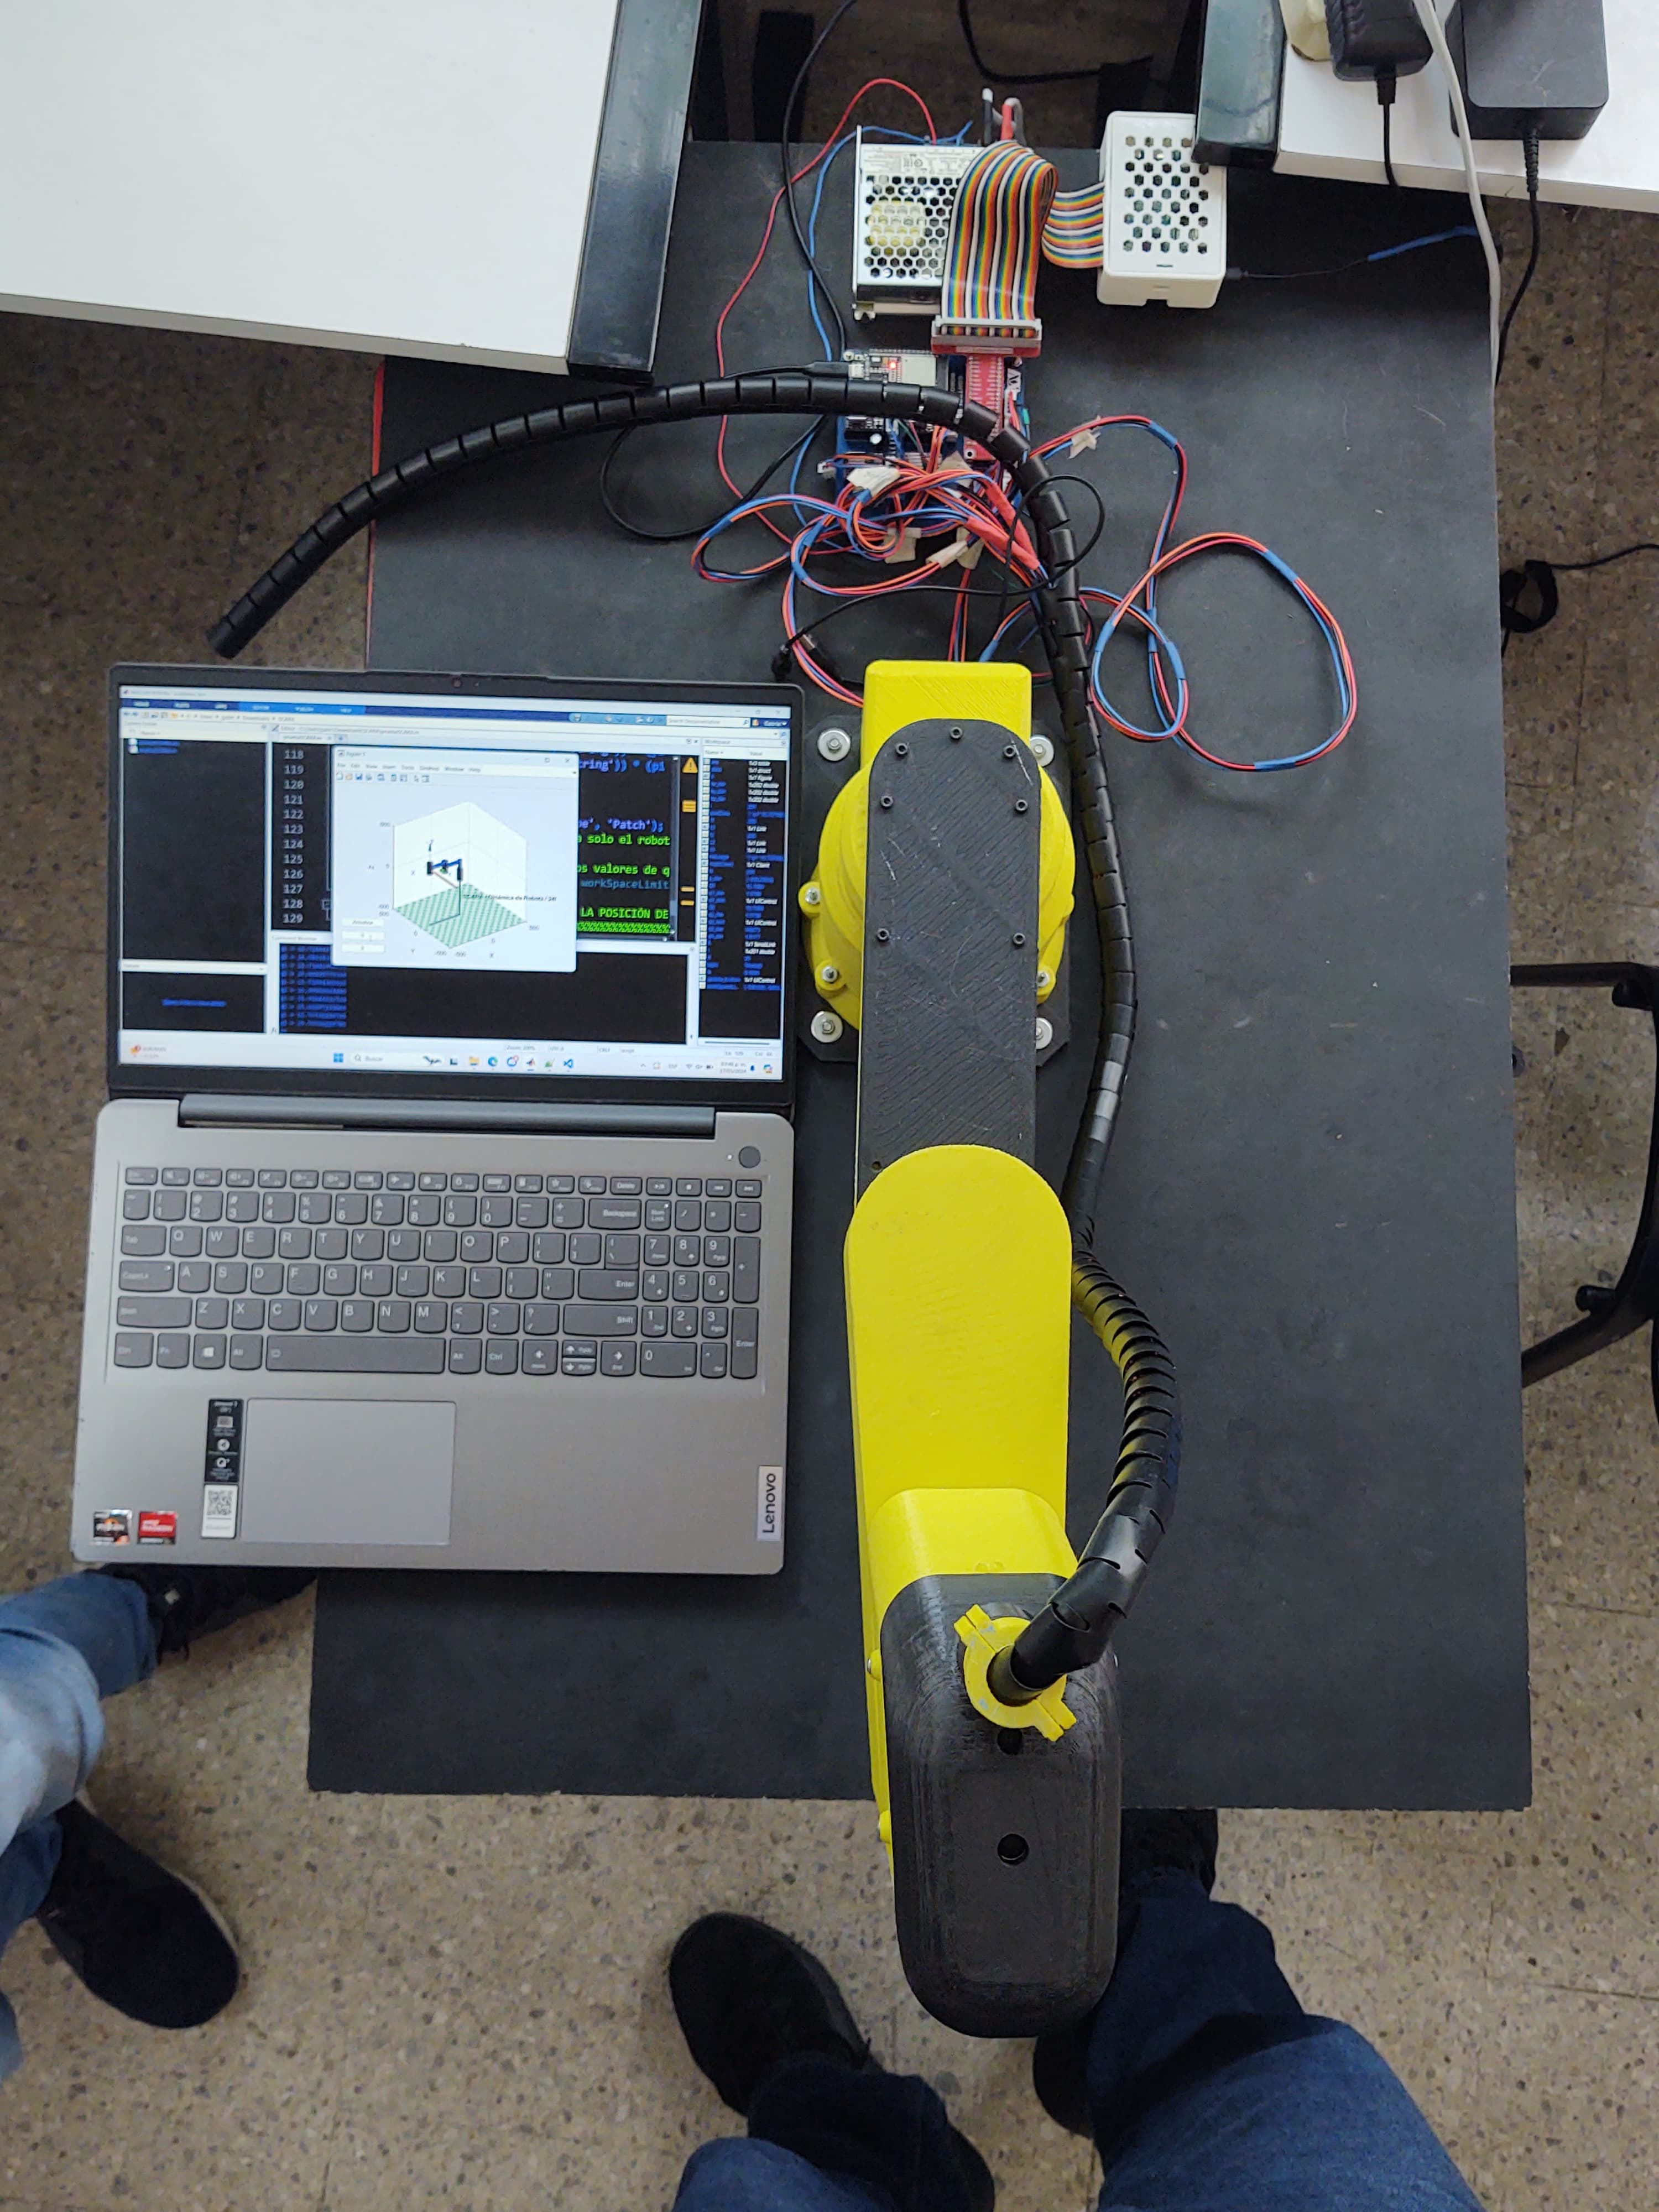
\includegraphics[width=0.45\textwidth]{SCARA3.jpg}
\caption{Componentes del Sistema que controla el robot SCARA}
\label{fig:my_label}
\end{figure}

Tras la exitosa simulación en MATLAB, se procedió a adaptar el código a las características del robot SCARA real proporcionado por la UAM Azcapotzalco. Este proceso involucró:

\begin{enumerate}
\item Medición de las dimensiones del robot: Se midieron con precisión las dimensiones del robot real para ajustar los parámetros del modelo utilizado en la simulación.
\item Integración con el hardware del robot: Se trabajó en conjunto con el equipo de Mekatronika UAM para integrar el software de control con el hardware del robot. Esto incluyó la configuración de la comunicación entre el microcontrolador ESP32 y el robot. El sistema completo de control para el robot SCARA incluye los siguientes componentes:
    \begin{enumerate}
    \item Microcontrolador ESP32: El ESP32, un microcontrolador versátil con conectividad WiFi y Bluetooth, se utiliza para enviar y recibir comandos de control al robot.
    \item Raspberry Pi: La Raspberry Pi actúa como servidor e intermediario entre el ESP32 y el software de control, facilitando la comunicación y el procesamiento de datos.
    \item Software Node-RED: Node-RED, una herramienta de programación basada en flujo, se utiliza para diseñar y gestionar el flujo de datos entre el ESP32, la Raspberry Pi y el dashboard.
    \item Protocolo MQTT a través de Mosquitto: El protocolo MQTT, un protocolo de mensajería ligero ideal para dispositivos con recursos limitados, se utiliza en conjunto con el broker Mosquitto para facilitar la comunicación entre los componentes del sistema.
    \item Dashboard de Node-RED: El dashboard gráfico de Node-RED proporciona una interfaz visual para el control y monitoreo en tiempo real del robot SCARA.
    \item Zona WiFi en Windows 10: Se configura una zona WiFi en un sistema operativo Windows 10 para conectar de forma inalámbrica el ESP32 y la Raspberry Pi, asegurando la comunicación entre estos dispositivos.
    \end{enumerate}
\item Ajuste de la cinemática inversa: Se realizaron ajustes en el algoritmo de cinemática inversa para considerar las características específicas del robot real, como la fricción y las limitaciones físicas de las articulaciones.
\end{enumerate}

\subsection{III. IMPLEMENTACIÓN EN EL ROBOT REAL:}

\subsubsection{Adaptación del modelo del robot}
Una vez validada la simulación, se procedió a implementar el control en el robot real. Para ello, se utilizaron las siguientes tecnologías:

\begin{enumerate}
\item IoT: El Internet de las Cosas (IoT) se utiliza para conectar los dispositivos físicos (ESP32, Raspberry Pi y robot SCARA) a través de una red inalámbrica.
\item JSON: El formato JSON se utiliza para empaquetar y transmitir datos entre los componentes del sistema.
\item MQTT: El protocolo MQTT, como se mencionó anteriormente, se utiliza para la comunicación entre los dispositivos.
\end{enumerate}

El código desarrollado en la simulación se adaptó a las características del robot real, considerando factores como la precisión del movimiento, la velocidad de las articulaciones y la interacción con el entorno:

\begin{lstlisting}[language=Matlab]
clc
clear
close all
%%%%%%%%%%%%%%%%%%%%%%%%%%%%%%%%%%%%%%%%%%%%%%%%%%
%Parametros de conexion MQTT
topic = 'Matlab'; % Tema al que se publicara
mqttClient = mqttclient("mqtt://192.168.137.1:1883");% Direccion del broker MQTT
% Suscripcion al tema Matlab
try
subscribe(mqttClient, topic);
disp(['Suscrito al tema: ' topic]);
catch ME
disp(['Error al suscribirse al tema: ' ME.message]);
return;
end
%Fin de Parametros de conexion MQTT
\end{lstlisting}

\begin{figure}[h!]
\centering
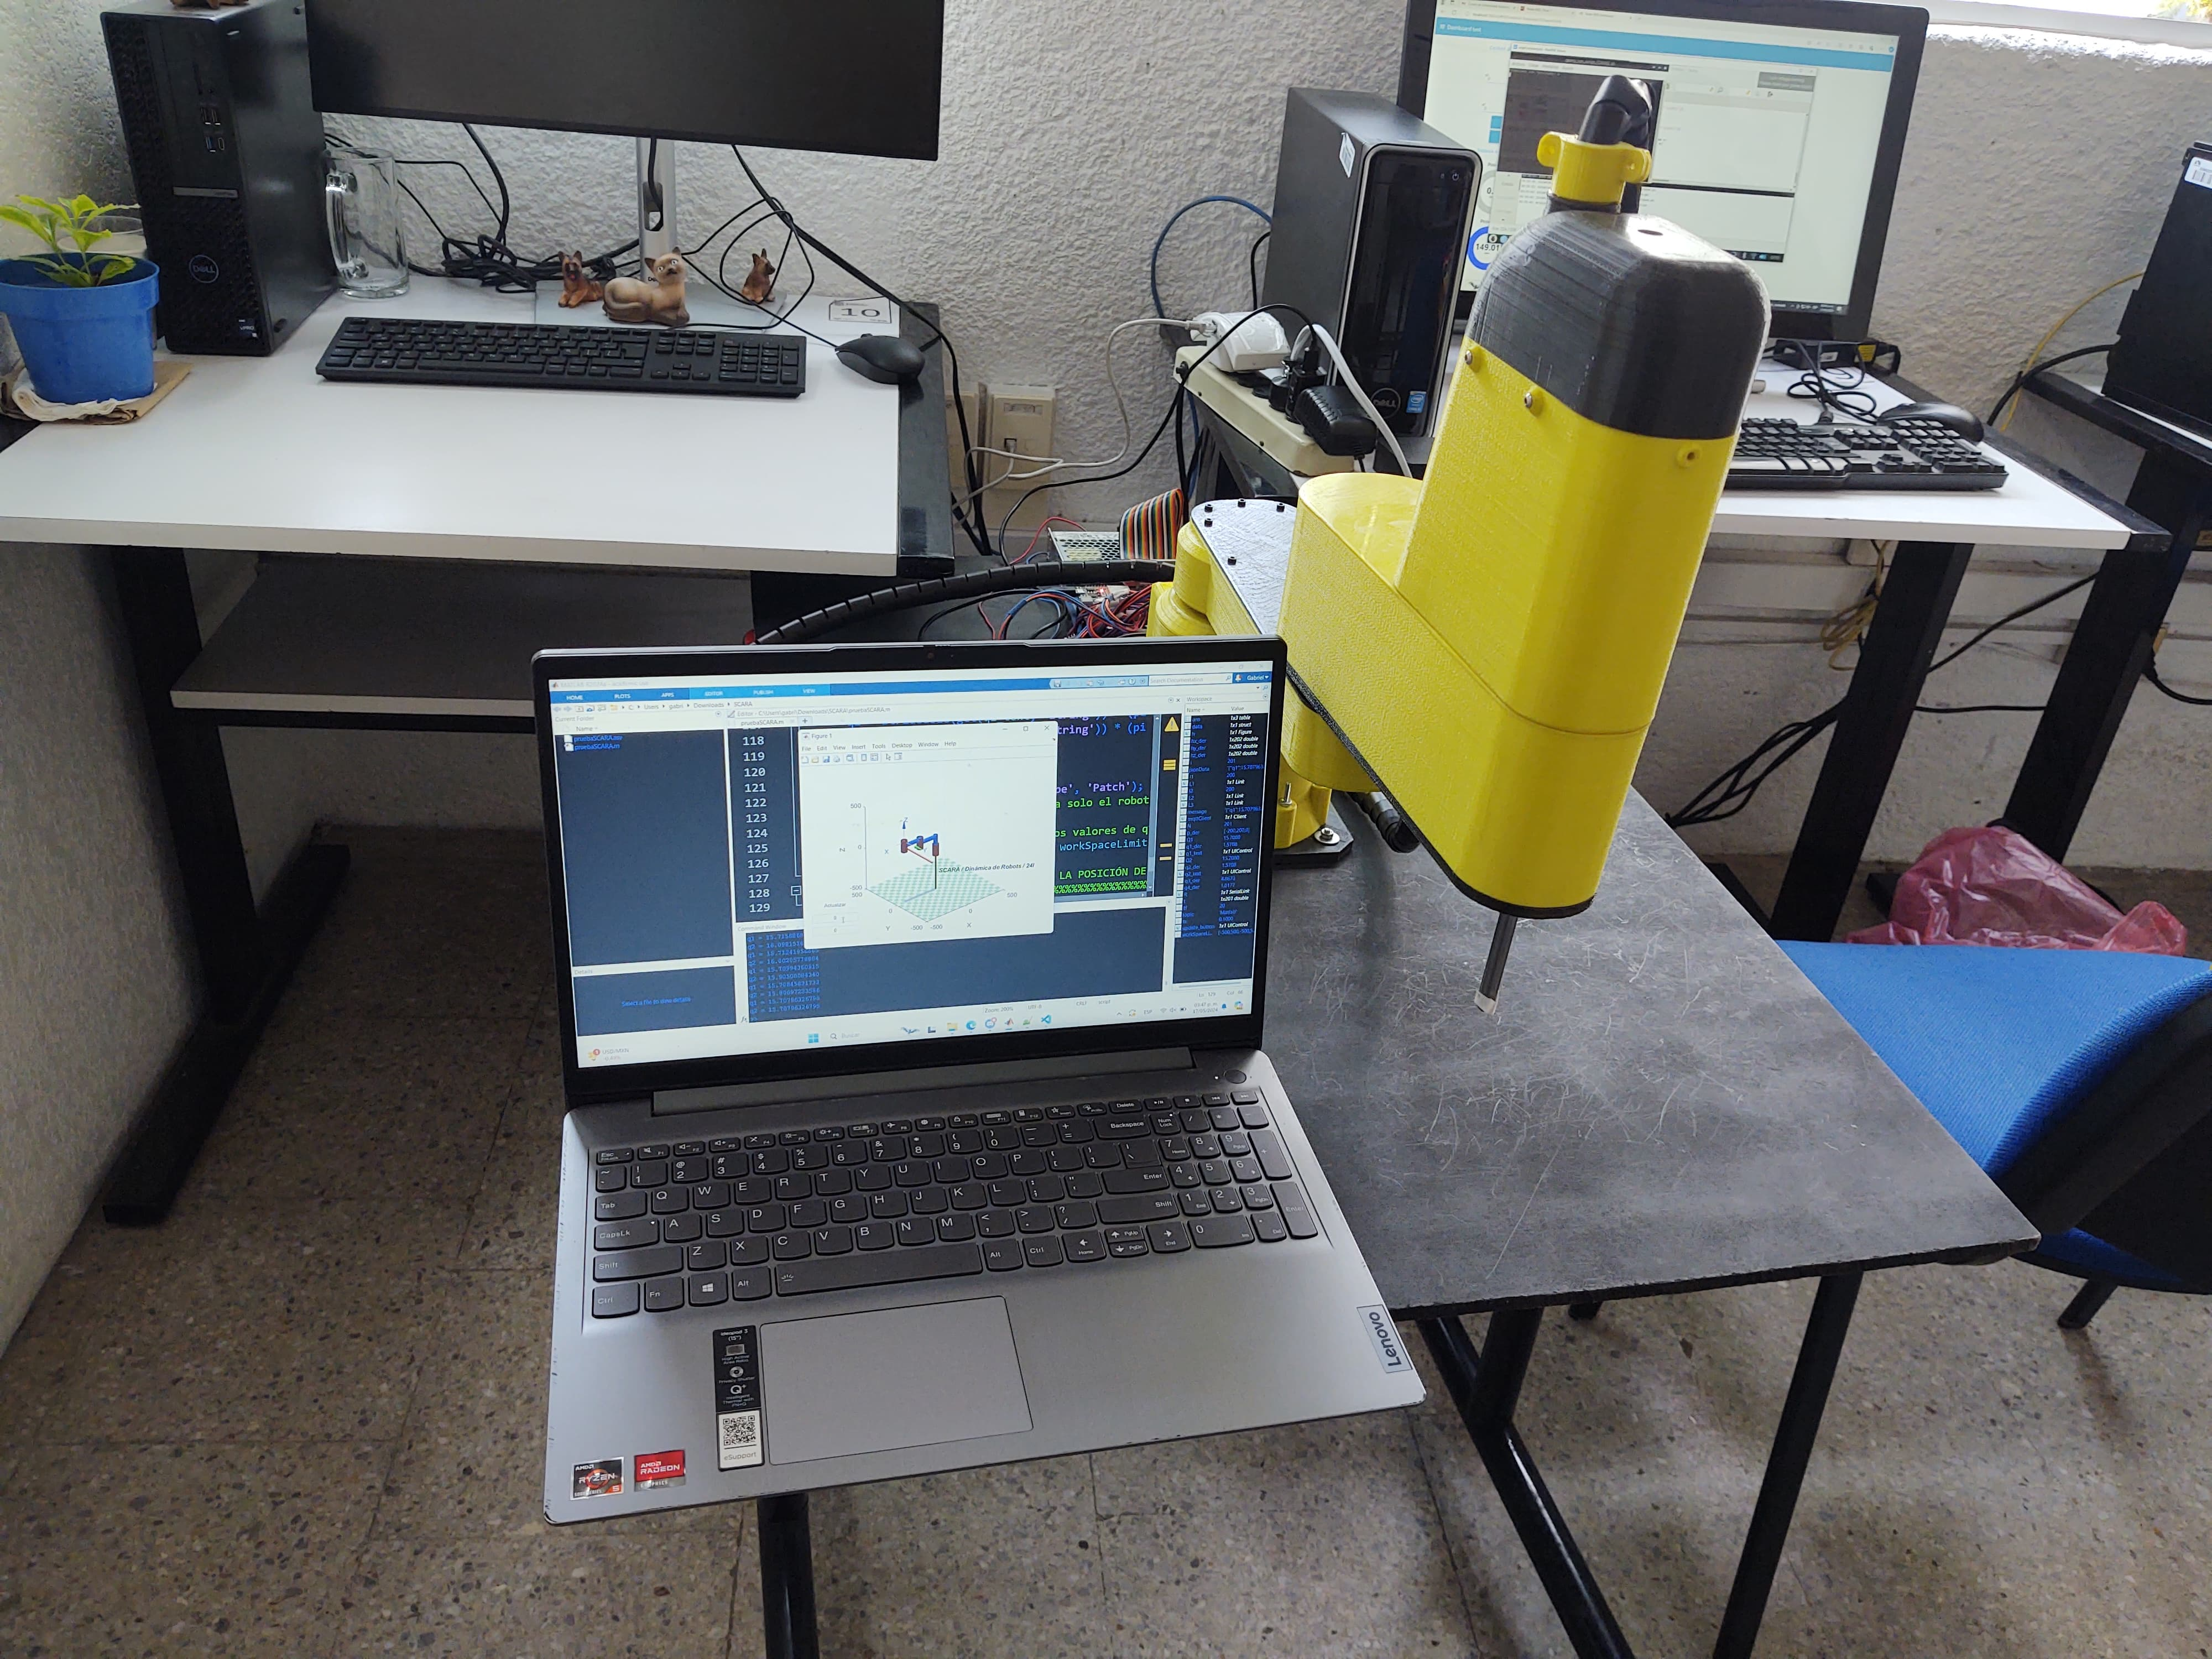
\includegraphics[width=0.45\textwidth]{SCARA4.jpg}
\caption{Simulación y visualización del Robot SCARA real.}
\label{fig:my_label}
\end{figure}

\begin{lstlisting}[language=Matlab]
%%%%%%%%%%%%%%%%%%%%%%%%%%%%%%%%%%%%%%%%%%%%%%%%%%
% CONSTRUCCION Y SIMULACION CON ROBOTICS TOOLBOX
% Definir las articulaciones
L1 = Link('d', 158, 'a', 200, 'alpha', 0);
L2 = Link('d', 43, 'a', 200, 'alpha', 0);
L3 = Link('d', 52, 'a', 0, 'alpha', 0);
% Simulacion del robot SCARA con sus dimensiones
global R;
R = SerialLink([L1, L2, L3], 'name', 'SCARA / Dinamica de Robots / 24I');
% Espacio de trabajo para visualizacion
global workSpaceLimits; % Declara workSpaceLimits como una variable global
workSpaceLimits = [-500 500 -500 500 -500 500];
% Posicion inicial del robot
global h; % Declara h como una variable global
if isempty(h) || ~isvalid(h) % Si la figura no existe o no es valida
h = figure; % Crea una nueva figura y guarda su identificador
end
figure(h); % Establece la figura del robot como la figura actual
R.plot([pi, 0, 0],'workspace', workSpaceLimits); % Cambia la posicion inicial a q1 = 180 grados
% FIN DE LA CONSTRUCCION Y SIMULACION CON ROBOTICS TOOLBOX
%%%%%%%%%%%%%%%%%%%%%%%%%%%%%%%%%%%%%%%%%%%%%%%%%%
\end{lstlisting}

\begin{figure}[h!]
\centering
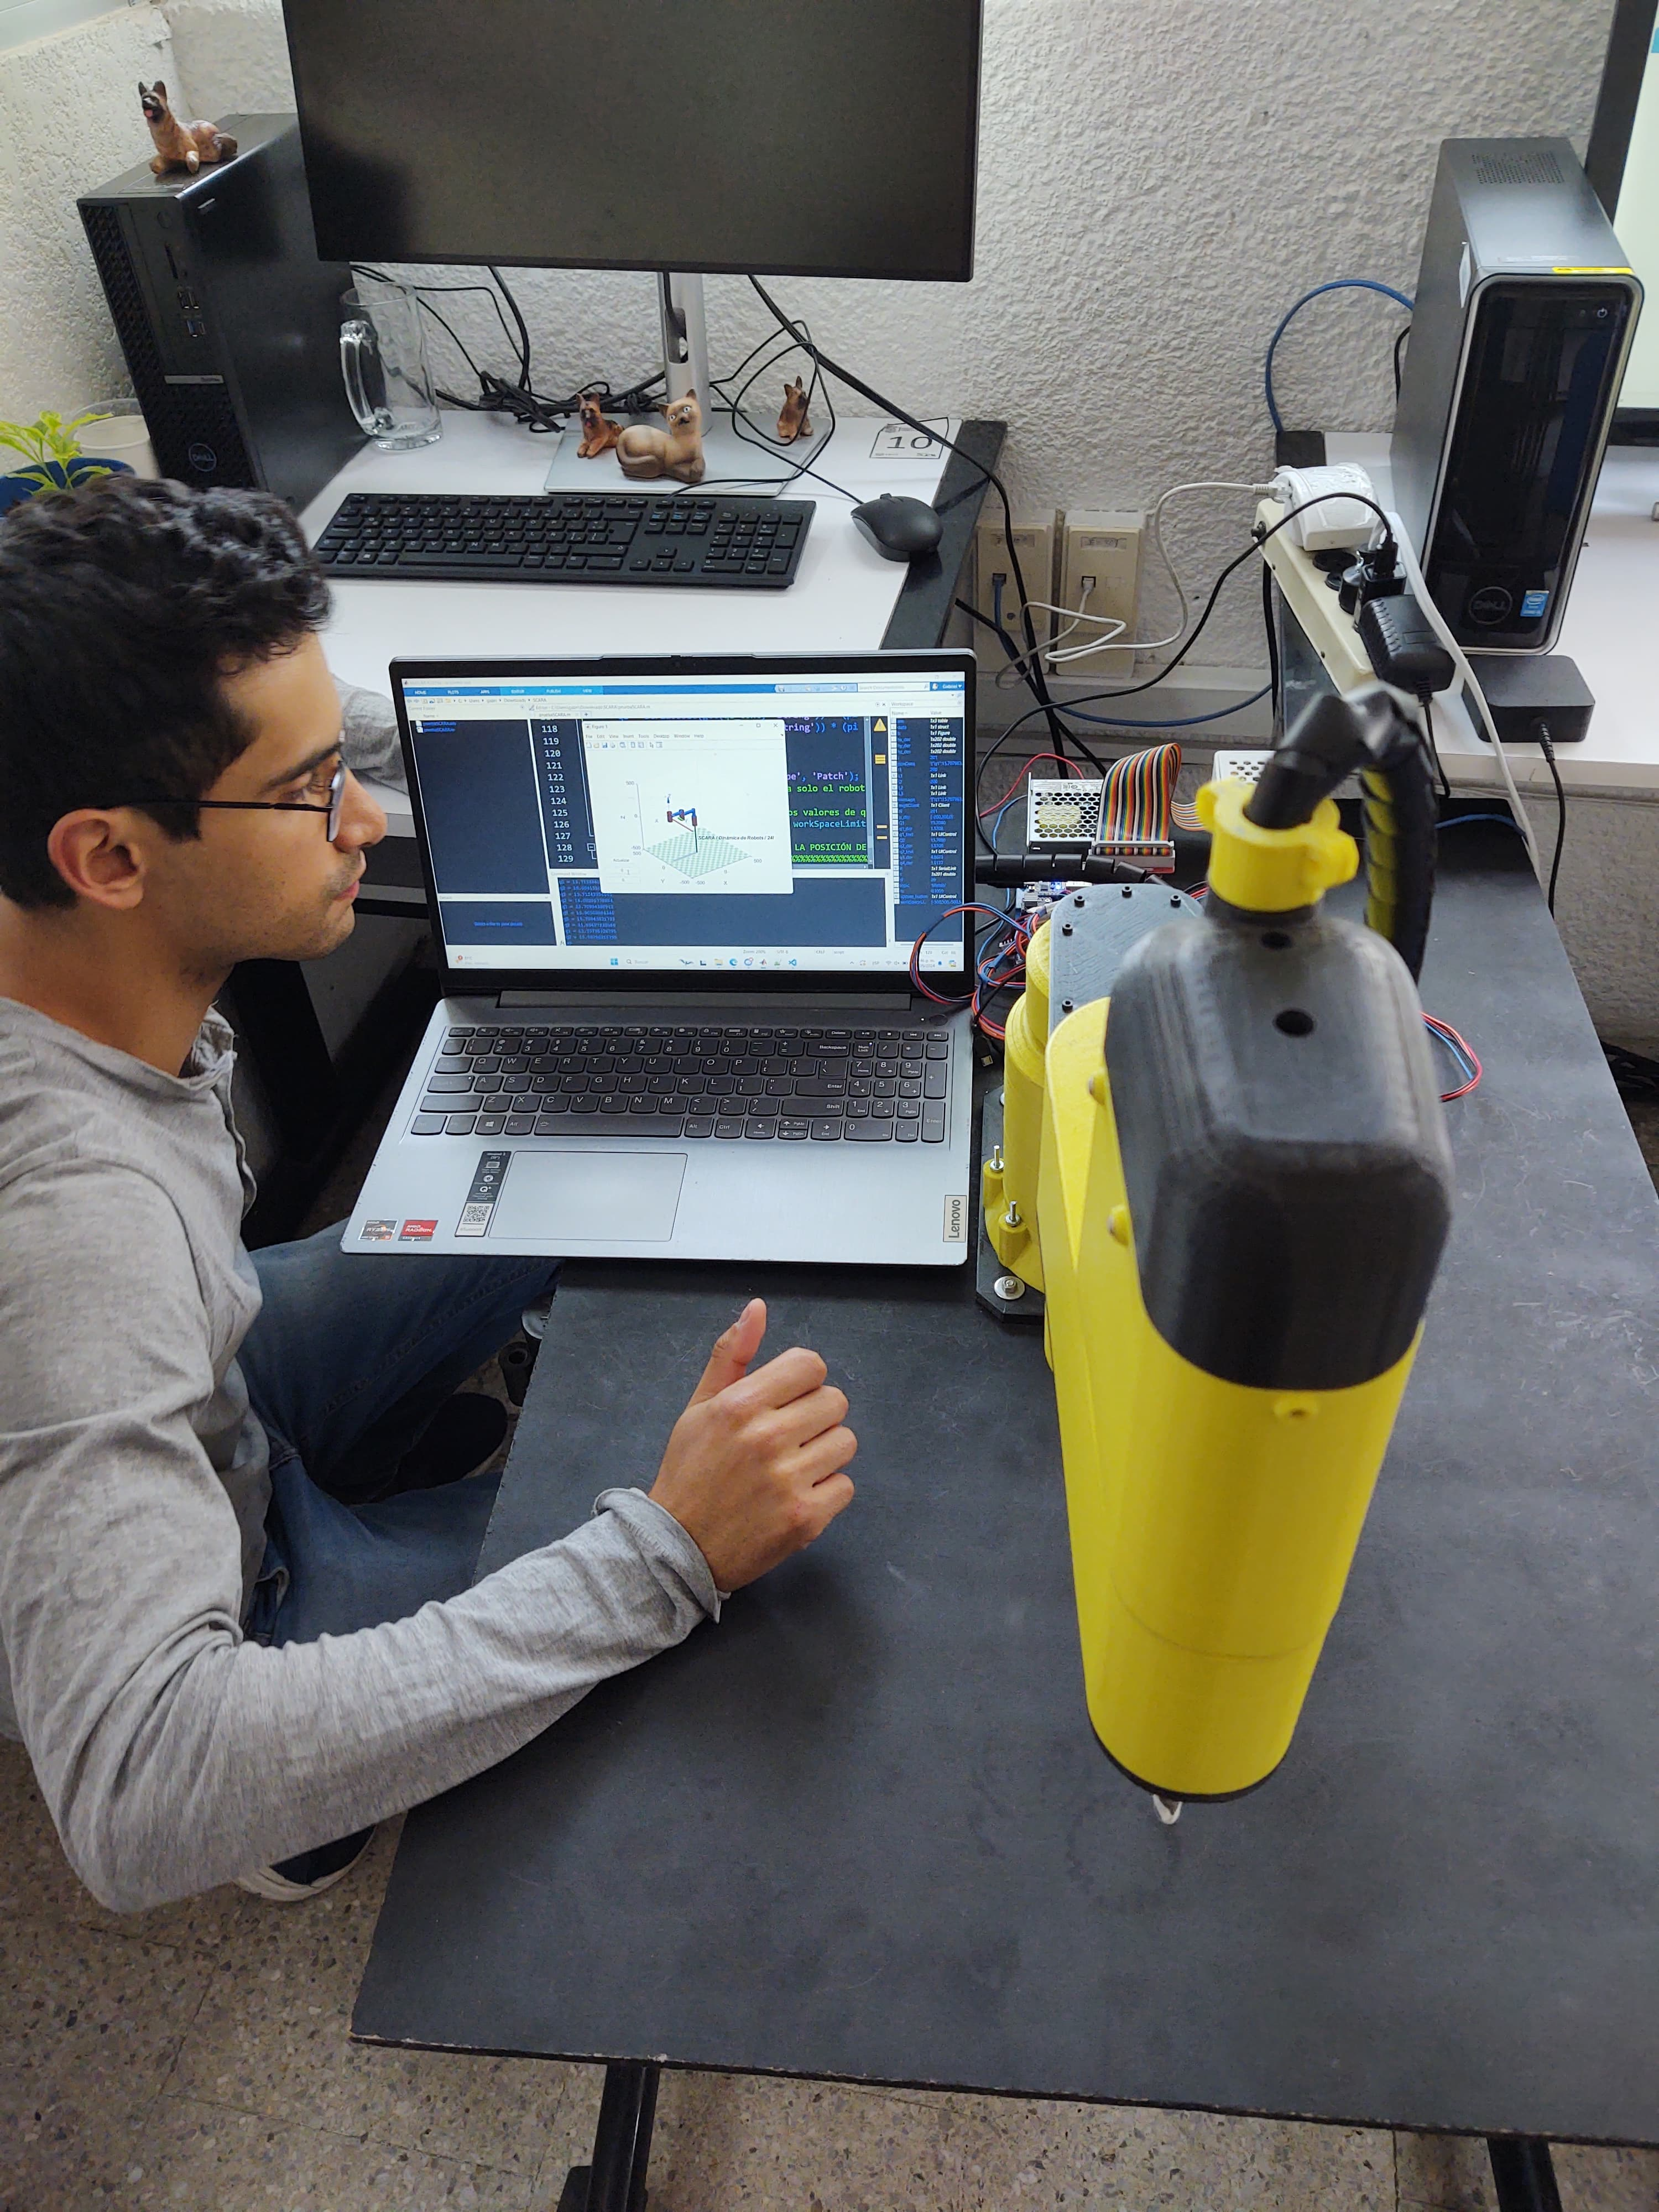
\includegraphics[width=0.45\textwidth]{SCARA5.jpg}
\caption{Simulación y movimiento del Robot SCARA real.}
\label{fig:my_label}
\end{figure}

\begin{lstlisting}[language=Matlab]
% Longitudes de los eslabones, usadas en la cinematica inversa
l1 = L1.a;
l2 = L2.a;
tf = 20; % Tiempo final
ts = 0.1; % Paso de tiempo
t = 0:ts:tf; % Vector de tiempo
N = length(t); % Numero de puntos en el vector de tiempo
% Linea de abajo a arriba
hx_der = zeros(1,N+1); % Vector de coordenadas x del efector final
hy_der = zeros(1,N+1); % Vector de coordenadas y del efector final
hz_der = zeros(1,N+1); % Vector de coordenadas z del efector final
for i = 1:N
hx_der(i) = -200; % Coordenada x del efector final
hy_der(i) = -200 + (400/N) * i; % Coordenada y
hz_der(i) = 0;
end
% Dibuja la trayectoria (de abajo a arriba)
hold on;
for i = 1:N
[q1_der, q2_der] = inverse_kinematics(hx_der(i), hy_der(i), l1, l2);
% Resultados
% Calculo de q3 y q4 (ajusta estos valores segun tus necesidades)
q3_der = 30; % Grados
q4_der = 45; % Grados
Q1 = q1_der * 10; % Variable para enviar al robot
q1_der = mod(q1_der, 2*pi); % Asegura que q1 esta en el rango [0, 2*pi]
q2_der = mod(q2_der, 2*pi); % Asegura que q2 esta en el rango [0, 2*pi]
q3_der = mod(q3_der, 2*pi); % Asegura que q3 esta en el rango [0, 2*pi]
q4_der = mod(q4_der, 2*pi); % Asegura que q4 esta en el rango [0, 2*pi]
\end{lstlisting}

\begin{figure}[h!]
\centering
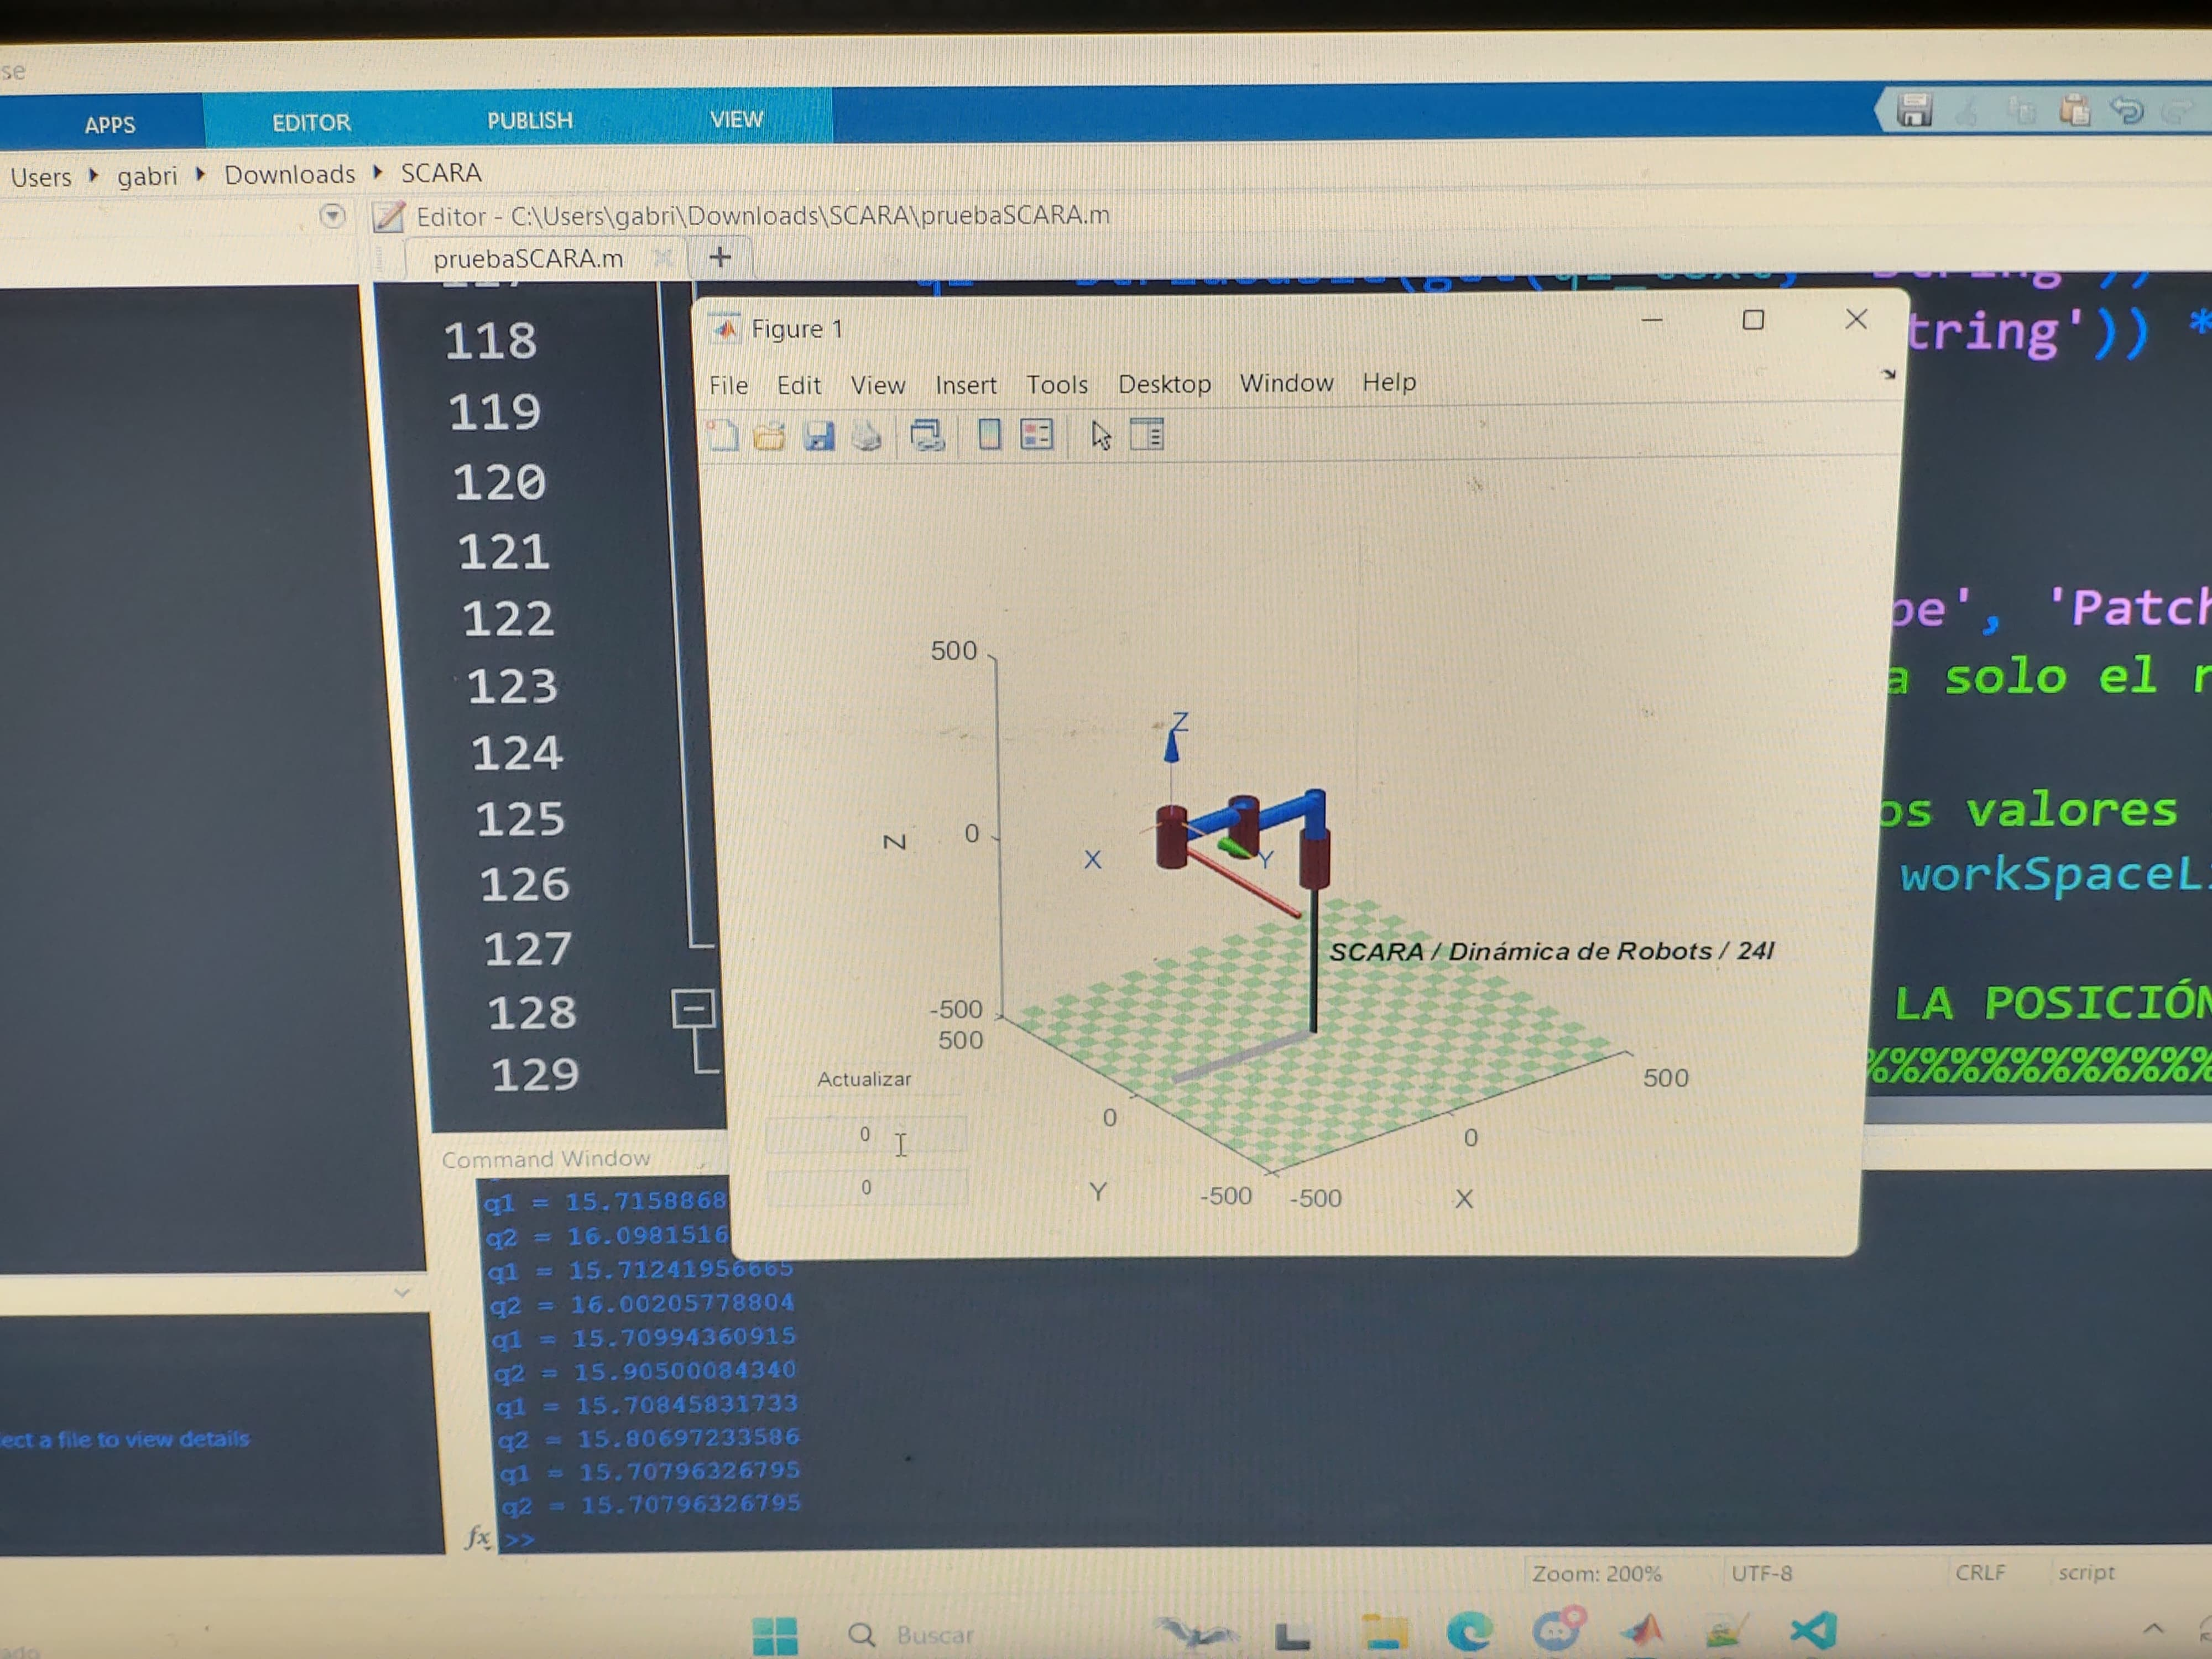
\includegraphics[width=0.45\textwidth]{SCARA6.jpg}
\caption{Envío de los párametros q1 y q2 generados mediante cinemática inversa (IK) y empaquedatos en un archivo JSON que se envía mediante MQTT al robot SCARA}
\label{fig:my_label}
\end{figure}

\begin{lstlisting}[language=Matlab]
% Empaquetamiento datos en estructura JSON
data = struct('q1', Q1, 'q2', q2_der, 'q3', q3_der, 'q4', q4_der);
jsonData = jsonencode(data);
% Publicacion del mensaje JSON al tema
message = jsonData;
write(mqttClient, topic, message); % Descomenta esta linea para enviar el mensaje
p_der = [hx_der(i), hy_der(i), hz_der(i)]; % Obtiene el punto actual de la trayectoria
plot_sphere(p_der, 10, 'r'); % Dibuja una esfera en el punto actual para visualizar la trayectoria (color verde)
R.plot([q1_der q2_der 0],'workspace', workSpaceLimits); % Color verde
fprintf("q1 = %.11f\n", q1_der);
fprintf("q2 = %.11f\n", q2_der);
drawnow;
end
hold off;
% Funcion de cinematica inversa
function [q1, q2] = inverse_kinematics(x, y, L1, L2)
% Calcula theta2
c2 = (x^2 + y^2 - L1^2 - L2^2) / (2 * L1 * L2);
if c2 < -1 || c2 > 1
error('El punto [%f, %f] esta fuera del alcance del robot.', x, y);
end
theta2 = acos(c2); % Solucion principal
% Calcula theta1
k1 = L1 + L2 * cos(theta2);
k2 = L2 * sin(theta2);
theta1 = atan2(y, x) - atan2(k2, k1);
% Asigna resultados a las variables de salida
q1 = theta1;
q2 = theta2;
end
\end{lstlisting}

\section{VII. Conclusión y Trabajo Futuro}

\textit{"El desarrollo de un Robot SCARA para Dibujar Letras Utilizando Cinemática Inversa en MATLAB ha permitido profundizar en la comprensión de los conceptos fundamentales de la robótica, como la cinemática inversa y el método Denavit-Hartenberg (DH), y su aplicación práctica en el diseño y control de robots." Ing. José Manuel Villa Vargas et al, 2024.}

Este proyecto ha sido posible gracias a la colaboración con la Universidad Autónoma Metropolitana (UAM) Azcapotzalco, a través del Departamento de Mecatrónica (Mekatronika UAM), quienes nos brindaron la oportunidad de trabajar con un robot SCARA real. La experiencia de llevar el código simulado a la práctica con el robot real ha sido invaluable para comprender los desafíos y las recompensas de la ingeniería robótica en el mundo real.

El robot SCARA, con su alta velocidad y precisión, es un excelente ejemplo de cómo la robótica puede ser utilizada para realizar tareas precisas y repetitivas. En este proyecto, se ha demostrado su capacidad para dibujar letras, lo que requiere un control preciso de la posición y orientación del efector final del robot.

El uso de la \textit{cinemática inversa}, que implica calcular las configuraciones articulares necesarias para que el efector final del robot alcance una posición y orientación deseadas, ha sido fundamental para lograr este objetivo. A través de la implementación de este concepto en MATLAB, se ha logrado controlar con éxito el robot al moverlo de una posición a otra, para después regresar a su posición inicial, simulando así la trayectoria de una línea recta.

Además, el método \textit{Denavit-Hartenberg (DH)}, un enfoque sistemático para describir la estructura cinemática de robots manipuladores, ha sido esencial para entender cómo se construye el robot SCARA y cómo se calcula la posición y orientación de cada eslabón del robot.

Este proyecto demuestra el potencial de los robots SCARA para realizar tareas de dibujo y escritura, abriendo nuevas posibilidades para su aplicación. Por ejemplo, estos robots podrían ser utilizados en la \textit{industria manufacturera} para marcar piezas, en la \textit{industria automotriz} para realizar soldaduras de precisión, o en el ámbito \textit{educativo} para enseñar conceptos de robótica a los estudiantes.

Este proyecto también abre la puerta a la exploración de robots SCARA más complejos. En el futuro, se podría investigar el uso de \textit{sensores de fuerza} para que el robot pueda interactuar con objetos de manera más delicada, o el desarrollo de \textit{algoritmos de control más avanzados} para que el robot pueda realizar tareas más complejas.

Para facilitar la comunicación y el control del robot SCARA, se implementaron tecnologías como \textit{MQTT} y \textit{Node-RED}. MQTT es un protocolo de mensajería ligero ideal para dispositivos con recursos limitados, como el ESP32, mientras que Node-RED es una herramienta de programación basada en flujo que permite diseñar y gestionar el flujo de datos entre los dispositivos. La integración de estas tecnologías ha permitido un control preciso y en tiempo real del robot SCARA.

En resumen, este proyecto ha sido una experiencia enriquecedora que ha permitido profundizar en los conceptos de la robótica y aplicarlos en un entorno real. La colaboración con la UAM Azcapotzalco fue fundamental para el éxito del proyecto, y esperamos continuar trabajando con ellos en el futuro para explorar nuevas aplicaciones de la robótica industrial.


\begin{figure}[h!]
\centering
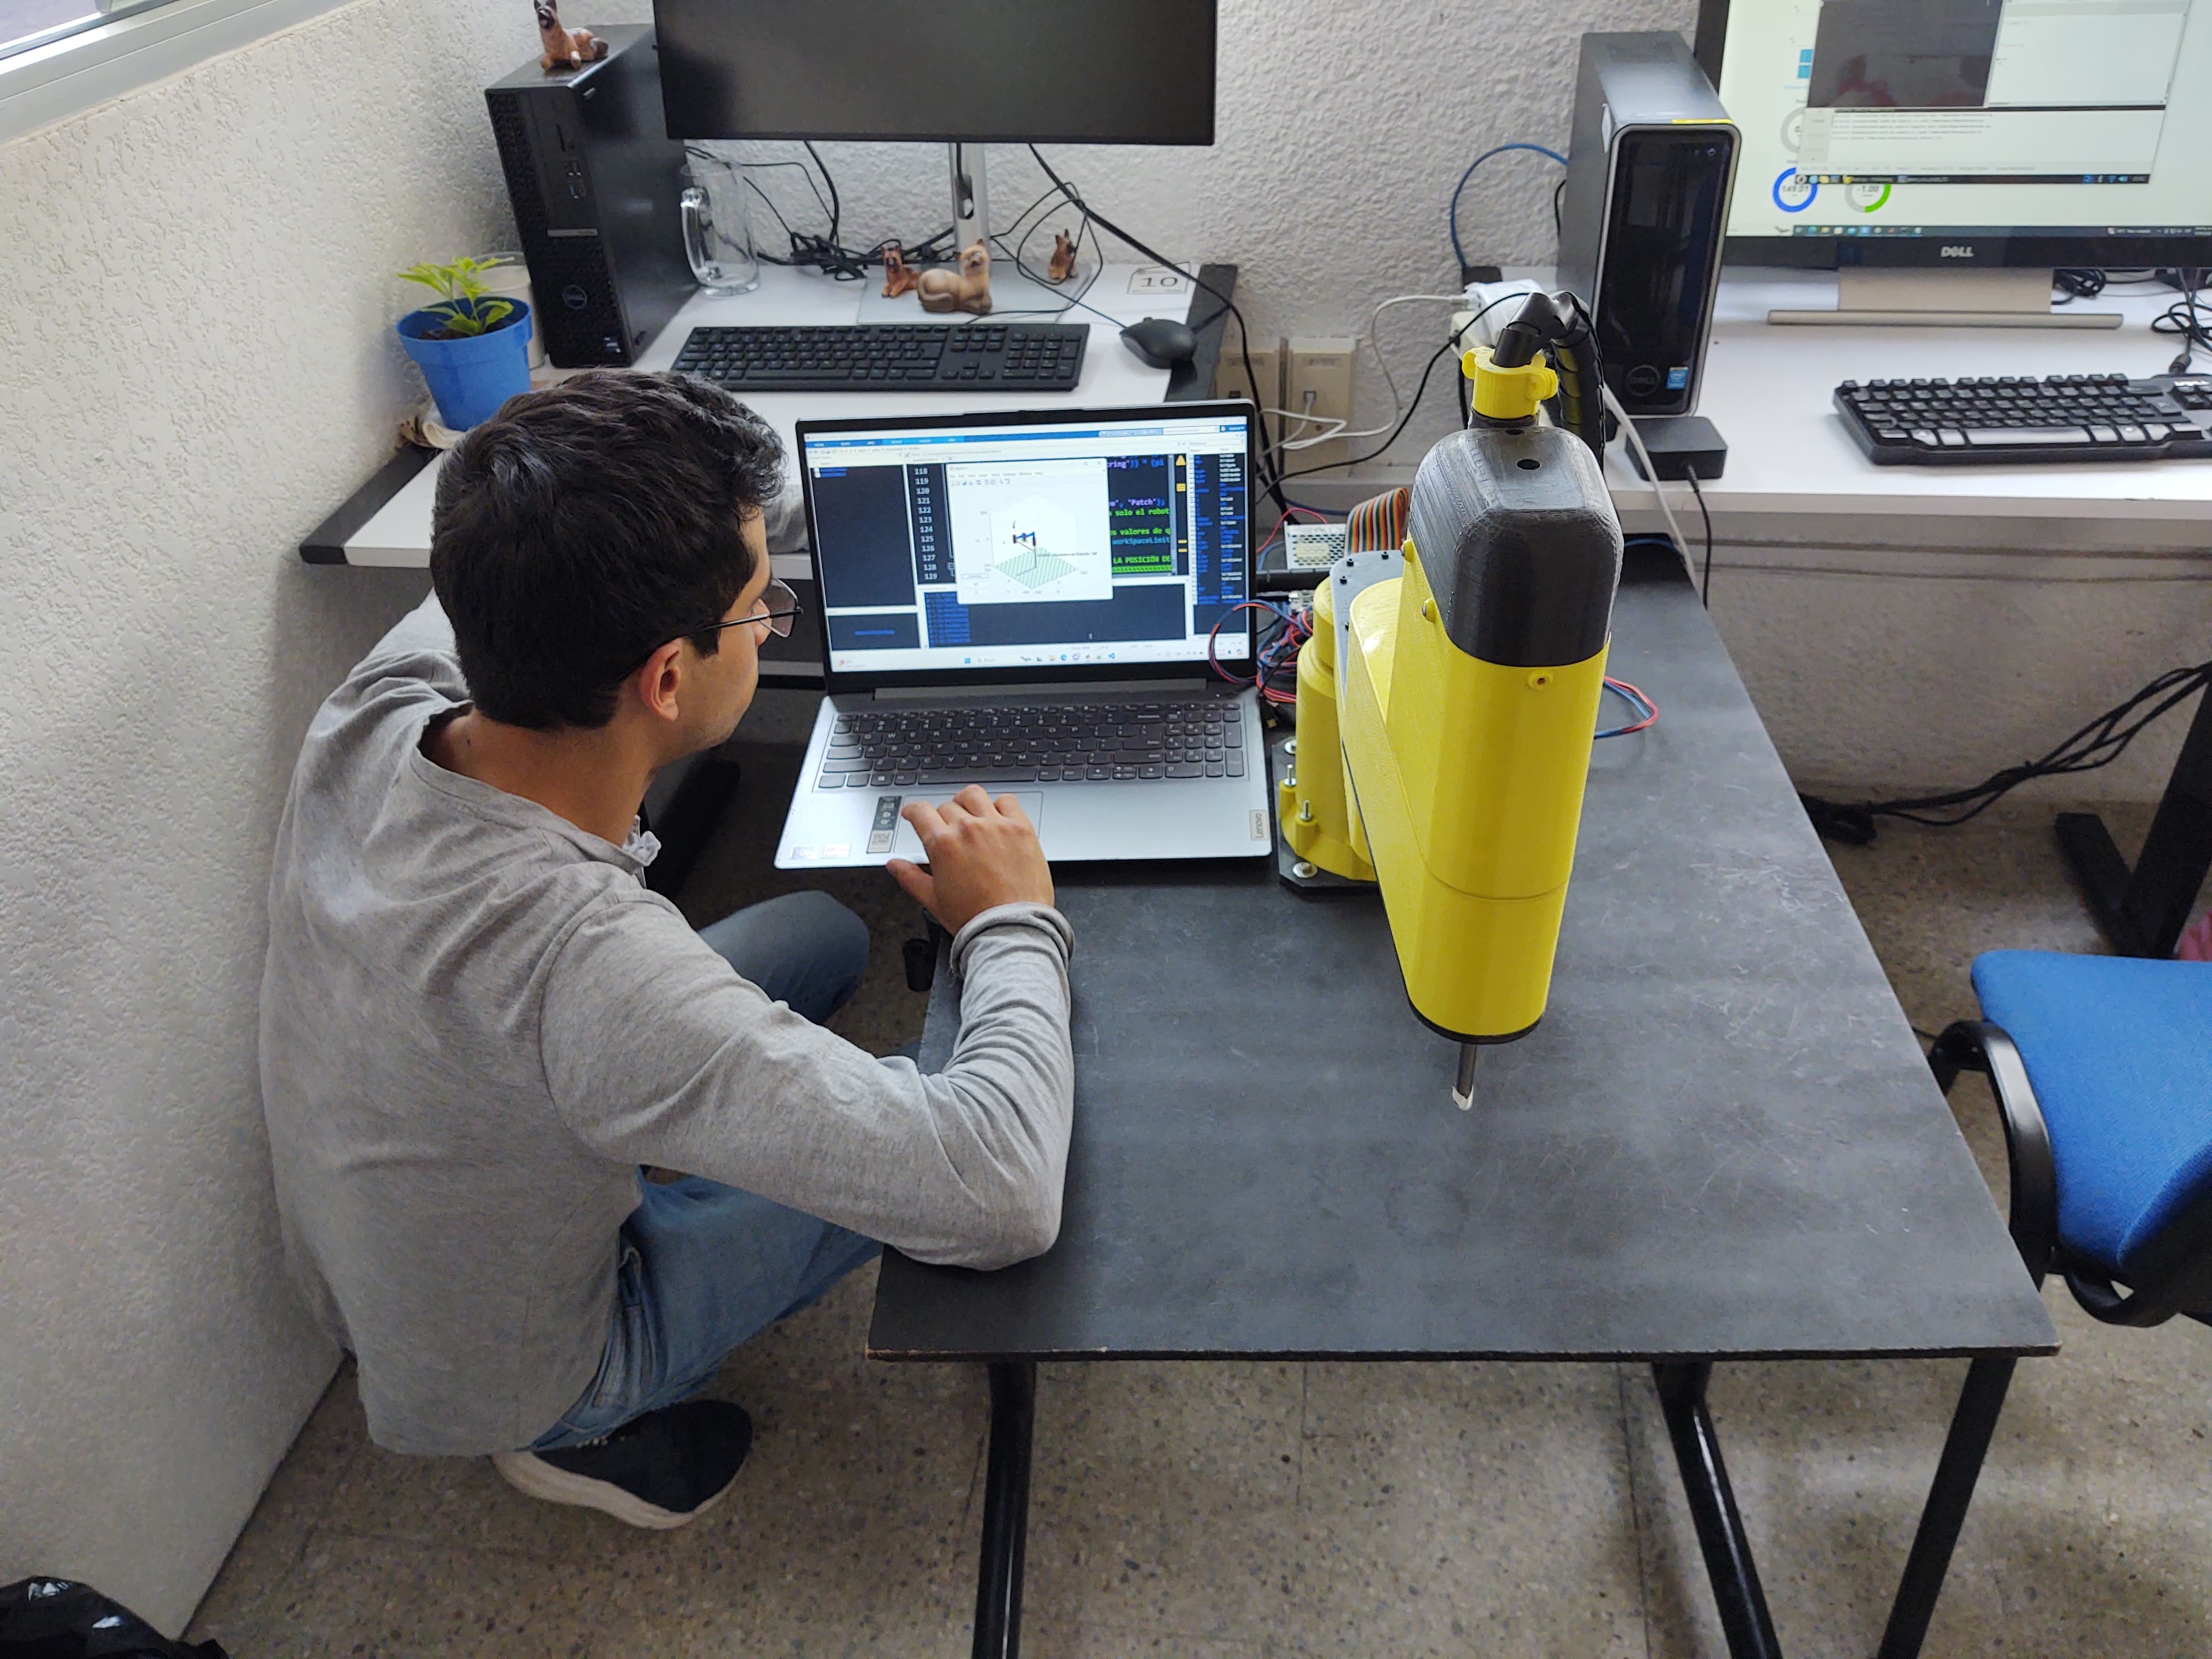
\includegraphics[width=0.45\textwidth]{SCARA7.jpg}
\caption{Adaptación de los hiper-parámetros en la simulación basándose en el robot SCARA real}
\label{fig:my_label}
\end{figure}

\begin{thebibliography}{9}

\bibitem[Corke(2020)]{1}
Peter Corke. (2020, April 27). Robotics Toolbox. Retrieved from \url{https://petercorke.com/toolboxes/robotics-toolbox/}

\bibitem[Universal Robots(n.d.)]{2}
Universal Robots. (n.d.). Collaborative robotic automation. Retrieved from \url{https://www.universal-robots.com/}

\bibitem[ASTESJ(2022)]{3}
Advances in Science, Technology and Engineering Systems Journal. (2022, September 5). Modelling and simulation of fuzzy-based coordination of trajectory planning and obstacle avoiding for RRP-Typed SCARA robots. Retrieved from \url{https://www.astesj.com/v06/i04/p39/}

\bibitem[Mathworks(n.d.)]{4}
Mathworks. (n.d.). Robotics System Toolbox documentation. Retrieved from \url{https://www.mathworks.com/help/robotics/}

\bibitem[IEEE Xplore(n.d.)]{5}
IEEE Xplore. (n.d.). Mechatronics Design and Kinematic Simulation of SCARA Robot to improve Safety and Time Processing of Covid-19 Rapid Test. Retrieved from \url{https://ieeexplore.ieee.org/document/9768506}

\bibitem[Review SCARA Robot(n.d.)]{6}
A review of SCARA Robot control System. (n.d.). Retrieved from \url{https://ieeexplore.ieee.org/abstract/document/9936755}

\bibitem[Pradhan et al.(2018)]{7}
Pradhan, S., Rajarajan, K., and Shetty, A. S. (2018). Prototype, emulation, implementation and evaluation of SCARA Robot in industrial environment. Procedia Computer Science, 133, 331–337. \url{https://doi.org/10.1016/j.procs.2018.07.041}

\bibitem[Grieco et al.(2014)]{8}
Grieco, L., Rizzo, A., Colucci, S., Sicari, S., Piro, G., Di Paola, D., and Boggia, G. (2014). IoT-aided robotics applications: Technological implications, target domains and open issues. Computer Communications, 54, 32–47. \url{https://doi.org/10.1016/j.comcom.2014.07.013}

\bibitem[Chanal et al.(2021)]{9}
Chanal, H., Guyon, J. B., Koessler, A., Dechambre, Q., Boudon, B., Blaysat, B., and Bouton, N. (2021). Geometrical defect identification of a SCARA robot from a vector modeling of kinematic joints invariants. Mechanism and Machine Theory, 162, 104339. \url{https://doi.org/10.1016/j.mechmachtheory.2021.104339}

\bibitem[Kinematic modeling(n.d.)]{10}
Kinematic modeling and simulation of an economical SCARA manipulator by Pro-E and verification using MATLAB/Simulink. (n.d.). Retrieved from \url{https://ieeexplore.ieee.org/abstract/document/7396410}

\end{thebibliography}

\end{document}